\blankpage
\pagestyle{indice}

{\centering{\includegraphics[width=130mm]{lettering.pdf}}}

\vspace{2.2cm}

%\begingroup\raggedleft
{\Formular{\huge{

\hspace*{7.5cm}\textit{\pageref{hedra}} \textbf{HEDRA}\\ %\vspace*{-.1cm}
\hspace*{8cm}\textit{\pageref{n-1}} \textbf{N-1 EDIÇÕES}\\ %\vspace*{-.1cm}
\hspace*{8cm}\textit{\pageref{circuito}} \textbf{CIRCUITO}\\ %\vspace*{-.1cm}
\hspace*{8cm}\textit{\pageref{kalinka}} \textbf{KALINKA}\\ %\vspace*{-.1cm}
\hspace*{8cm}\textit{\pageref{ima}} \textbf{ÍMÃ}\\ %\vspace*{-.1cm}
%\hspace*{8cm}\textit{\pageref{azougue}} \textbf{AZOUGUE}\\ %\vspace*{-.1cm}
\hspace*{8cm}\textit{\pageref{ayllon}} \textbf{AYLLON}\\ %\vspace*{-.1cm}
\hspace*{8cm}\textit{\pageref{quadrado}} \textbf{$\square\fullmoon$.ORG}\\ %\vspace*{-.1cm}
}}}

%\endgroup

\hspace*{-7cm}\hrulefill\hspace*{-7cm}

\vspace{1cm}

\hspace*{-.5cm}\parbox{150pt}{\raggedright EdLab é um novo grupo editorial que atuará no mercado do livro, e reúne desde editoras com mais de vinte anos até novos selos editoriais independentes. Neste catálogo apresentamos os quarenta e oito lançamentos das sete editoras do grupo, disponibilizados ao mercado durante o terceiro trimestre de 2020, que abrange os meses de julho a setembro. Além de artes gráficas produzidas especialmente para a edição, o catálogo também conta com sete artigos, sendo alguns deles inéditos. Para mais informações e detalhes sobre os livros consulte o conteúdo interno.} %\enlargethispage{\baselineskip}

\pagebreak
\blankpage
\pagebreak

\pagestyle{grid}

\begin{figure}[!htbp]
\begin{tabular}{cccc}

\vspace{.5cm}
\hspace*{-.5cm}
\subfloat{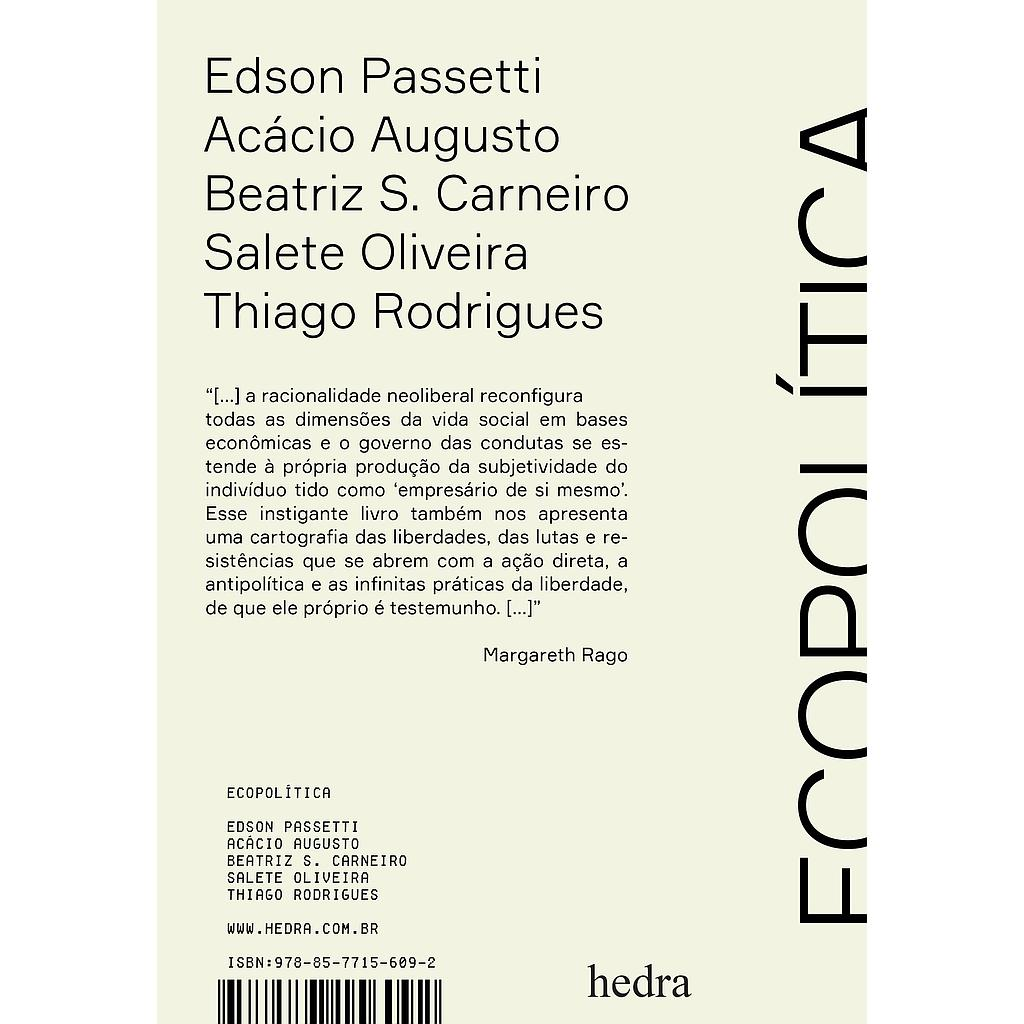
\includegraphics[width=46mm]{./grid/passetti.jpeg}}
\subfloat{
\includegraphics[width=46mm]{./grid/freud.png}}
\subfloat{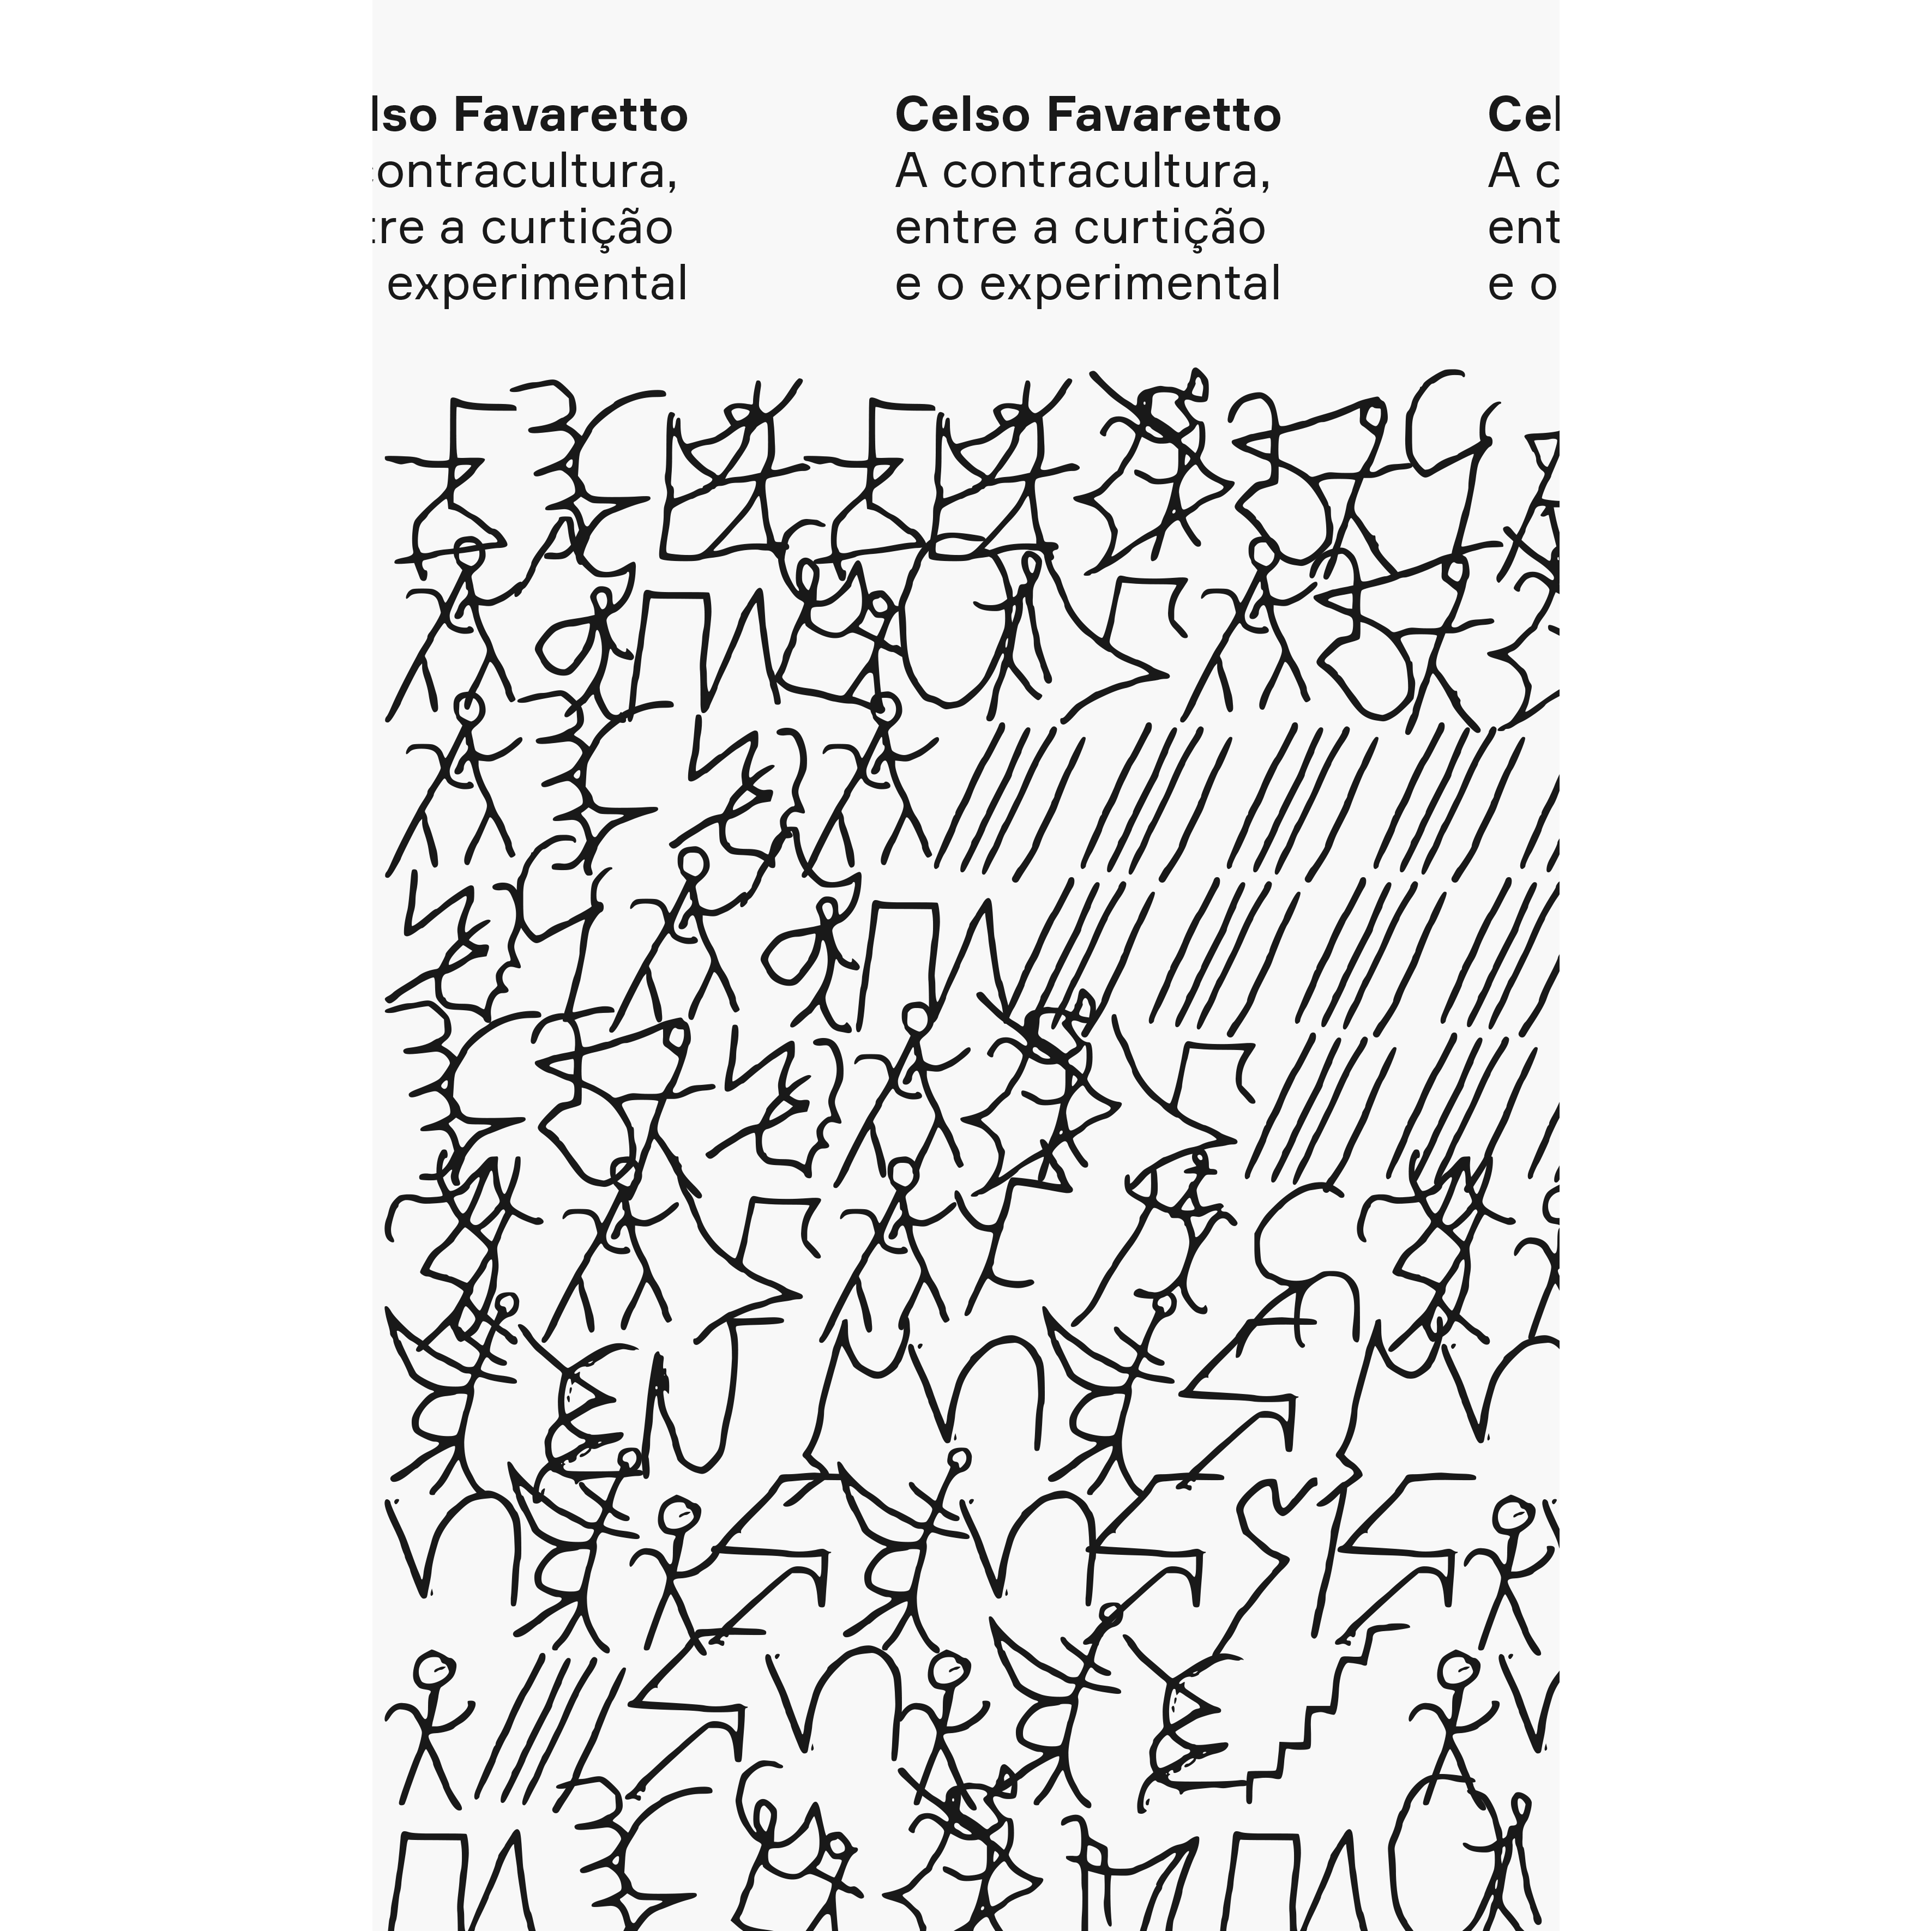
\includegraphics[width=46mm]{./grid/favaretto.png}}\\\hspace*{-.5cm}
\vspace{.5cm}
\subfloat{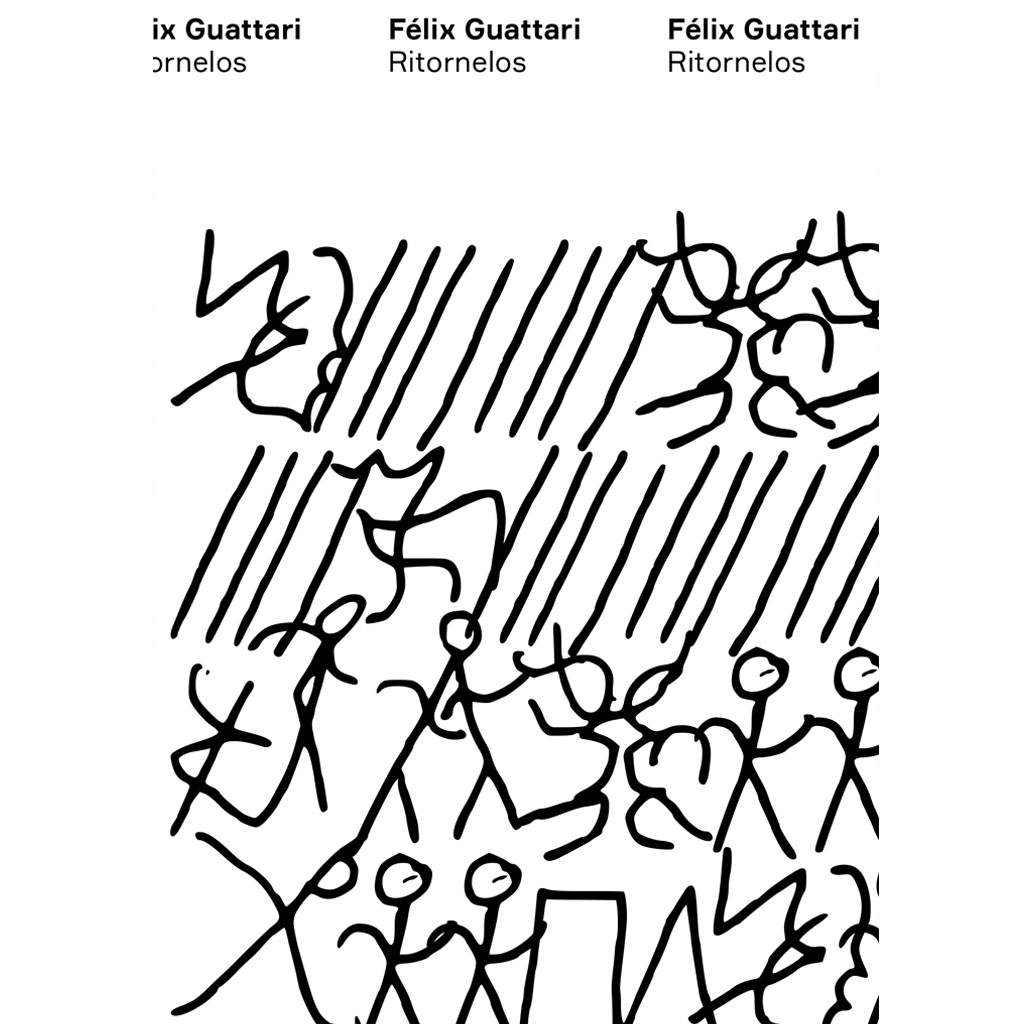
\includegraphics[width=46mm]{./grid/guattari.jpg}}
\subfloat{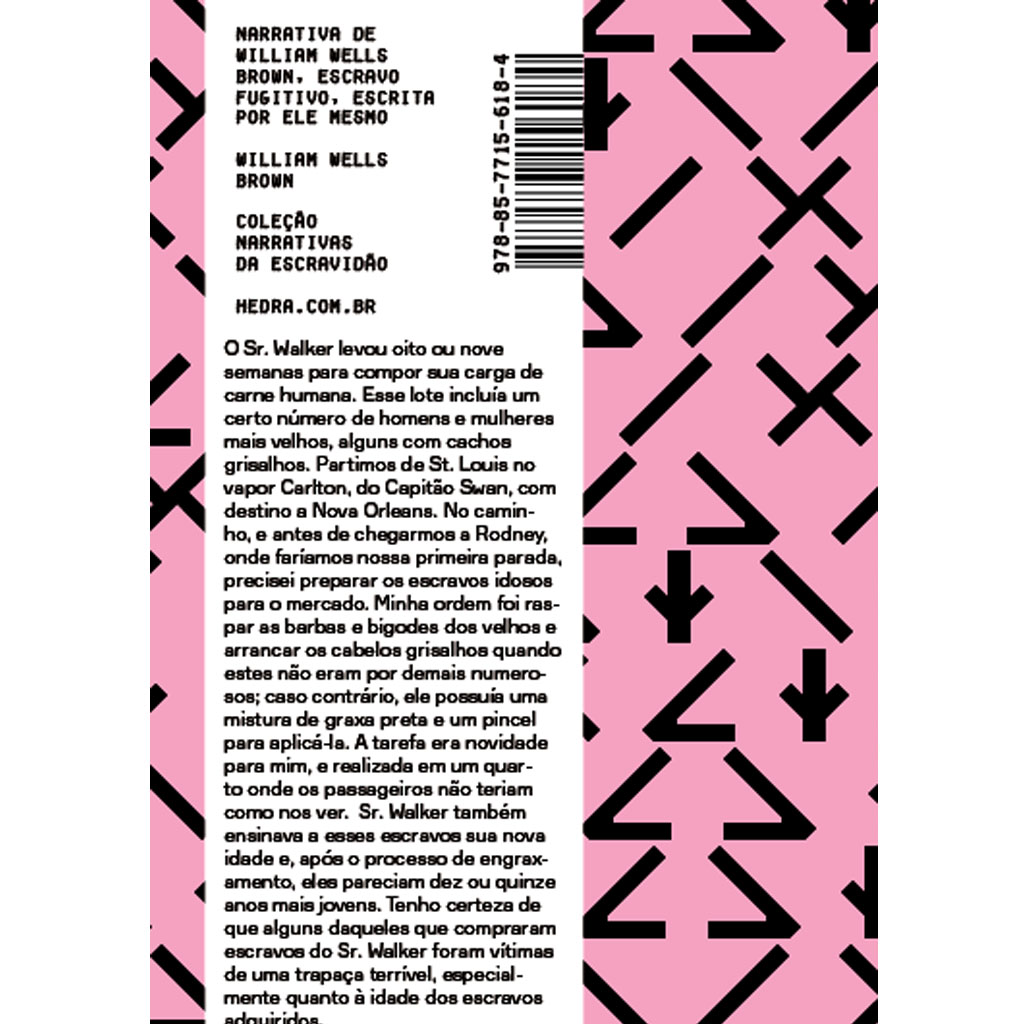
\includegraphics[width=46mm]{./grid/brown.jpg}}
\subfloat{
\includegraphics[width=46mm]{./grid/jacobs.jpg}}\\\hspace*{-.5cm}
\vspace{.5cm}
\subfloat{
\includegraphics[width=46mm]{./grid/wpa.jpg}}
\subfloat{
\includegraphics[width=46mm]{./grid/antifa.png}}
\subfloat{
\includegraphics[width=46mm]{./grid/soma.png}}\\\hspace*{-.5cm}
\vspace{.5cm}
\subfloat{
\includegraphics[width=46mm]{./grid/black.png}}
\subfloat{
\includegraphics[width=46mm]{./grid/robson.png}}
\subfloat{
\includegraphics[width=46mm]{./grid/jazz.jpg}}
\end{tabular}
\end{figure}

\pagebreak

\begin{figure}[!htbp]
\begin{tabular}{cccc}

\vspace{.5cm}
\hspace*{-.5cm}
\subfloat{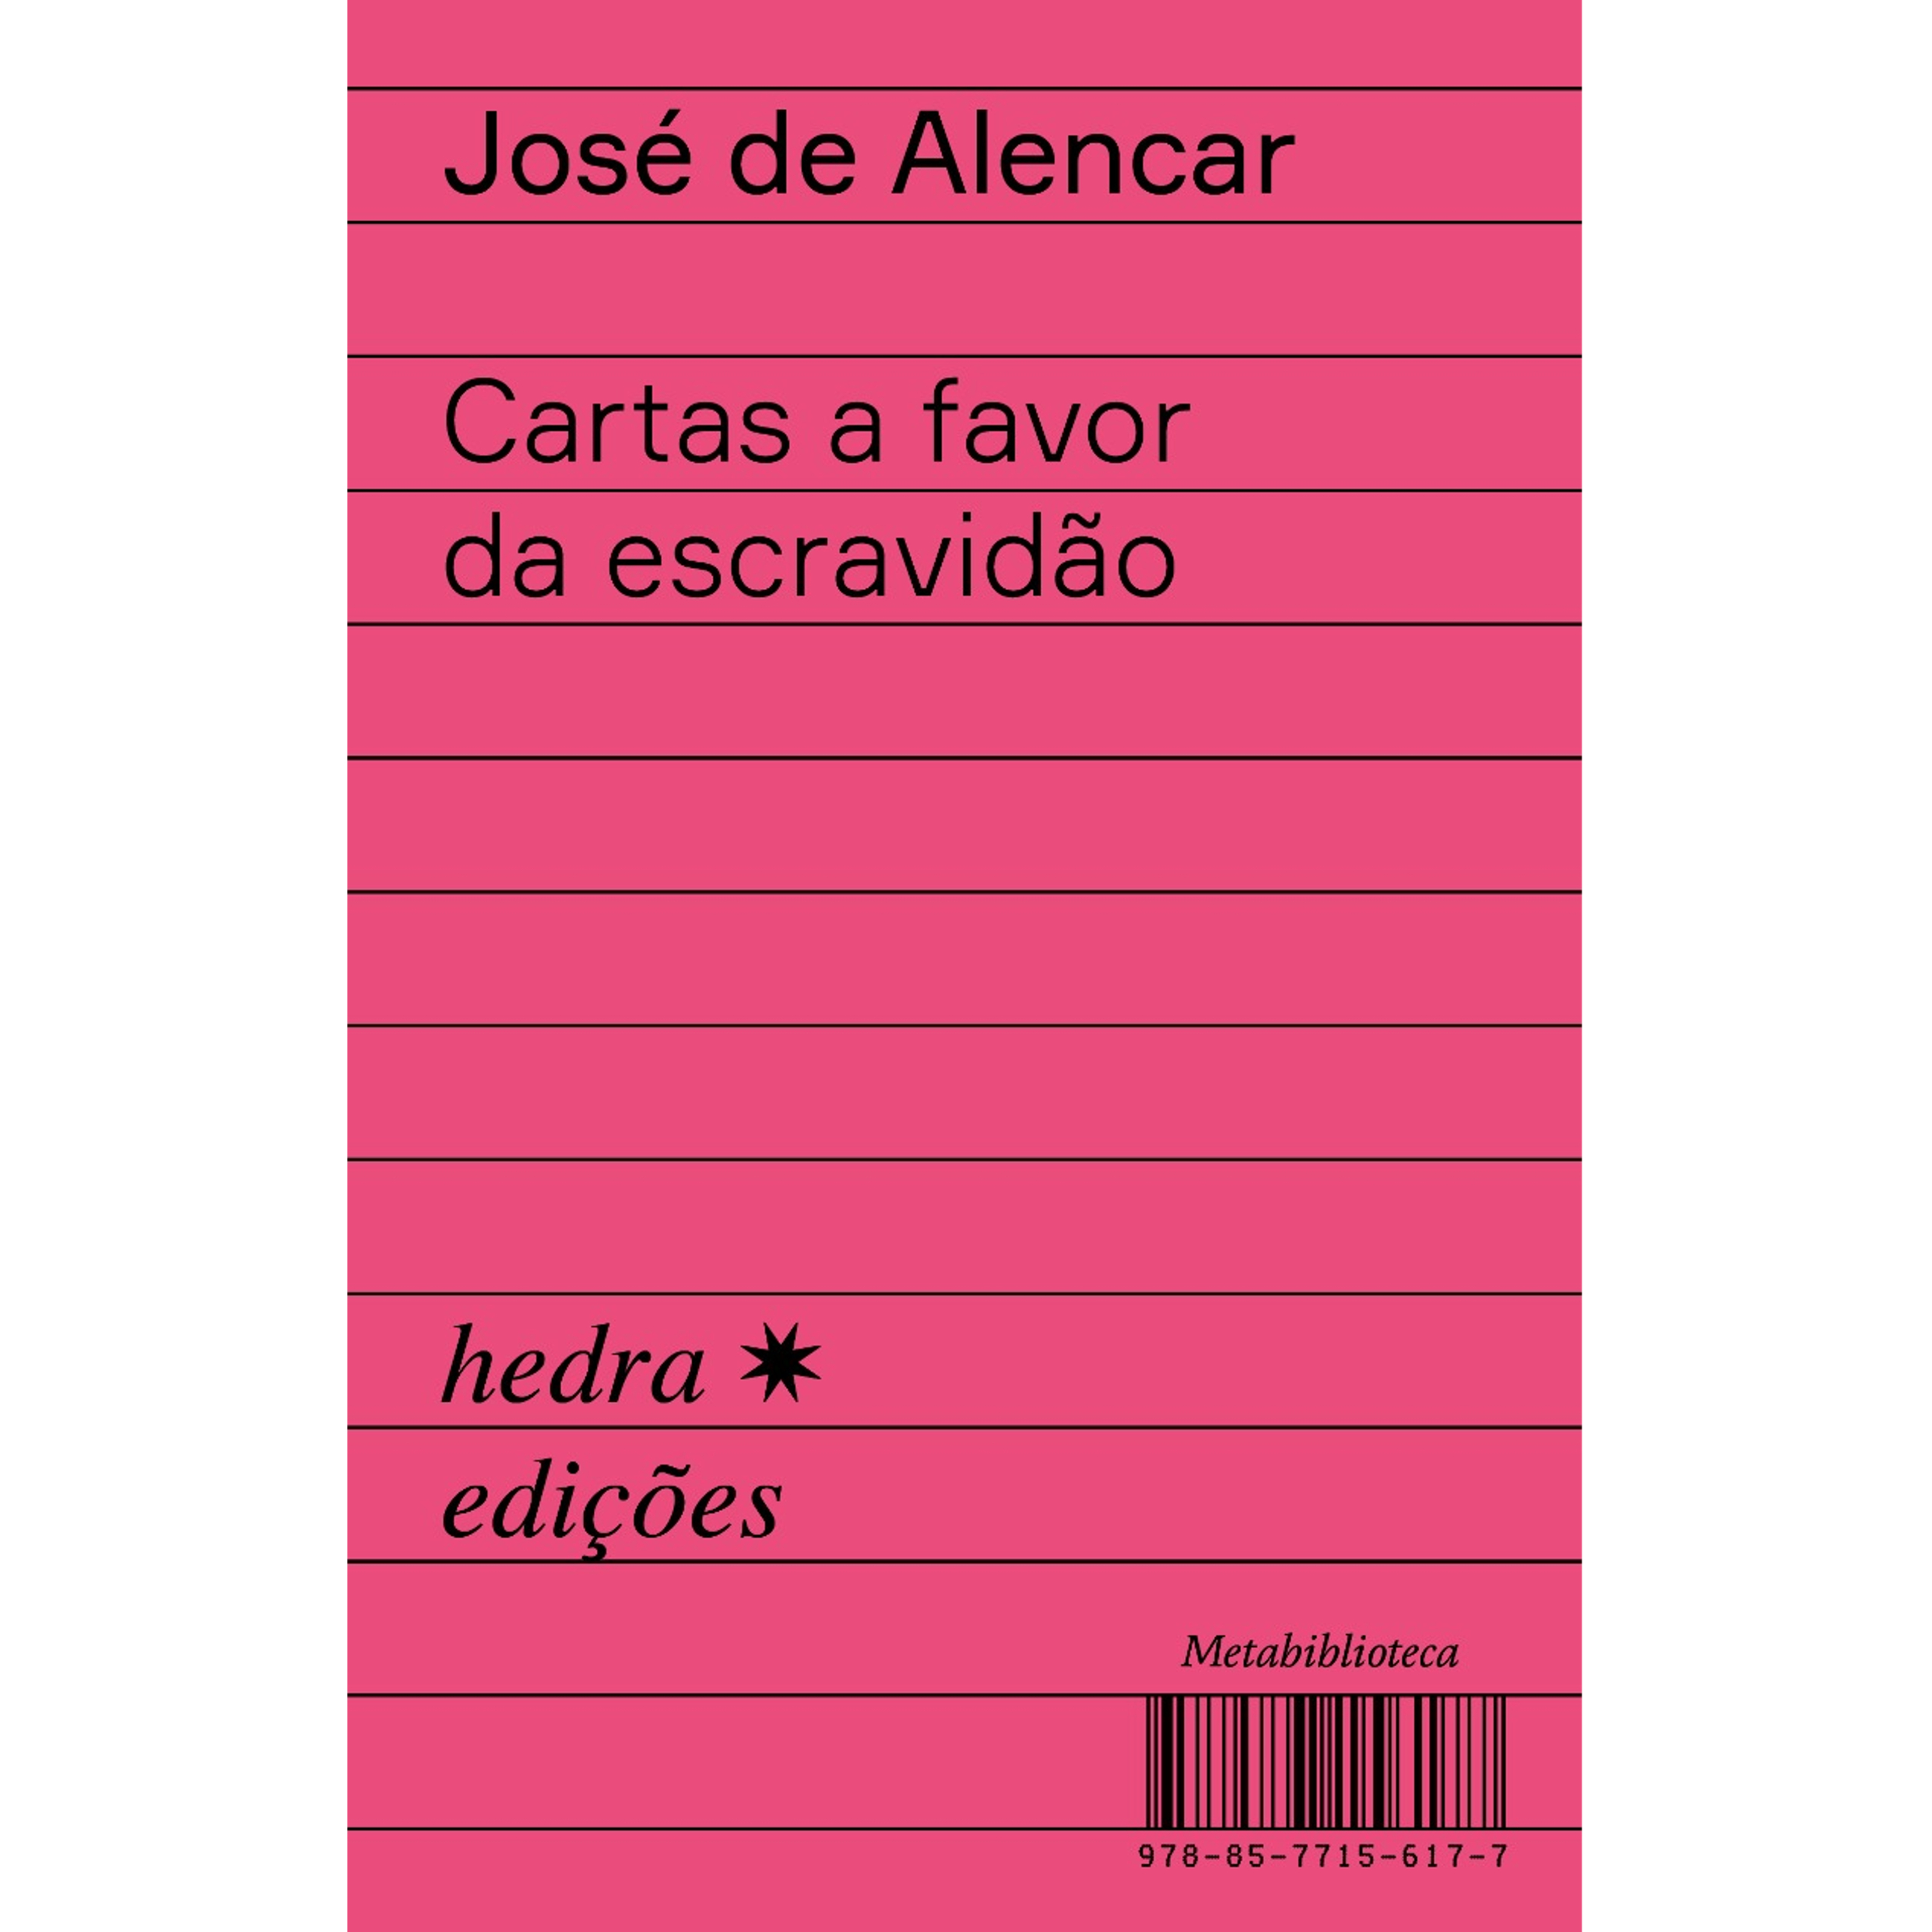
\includegraphics[width=46mm]{./grid/alencar.jpg}}
\subfloat{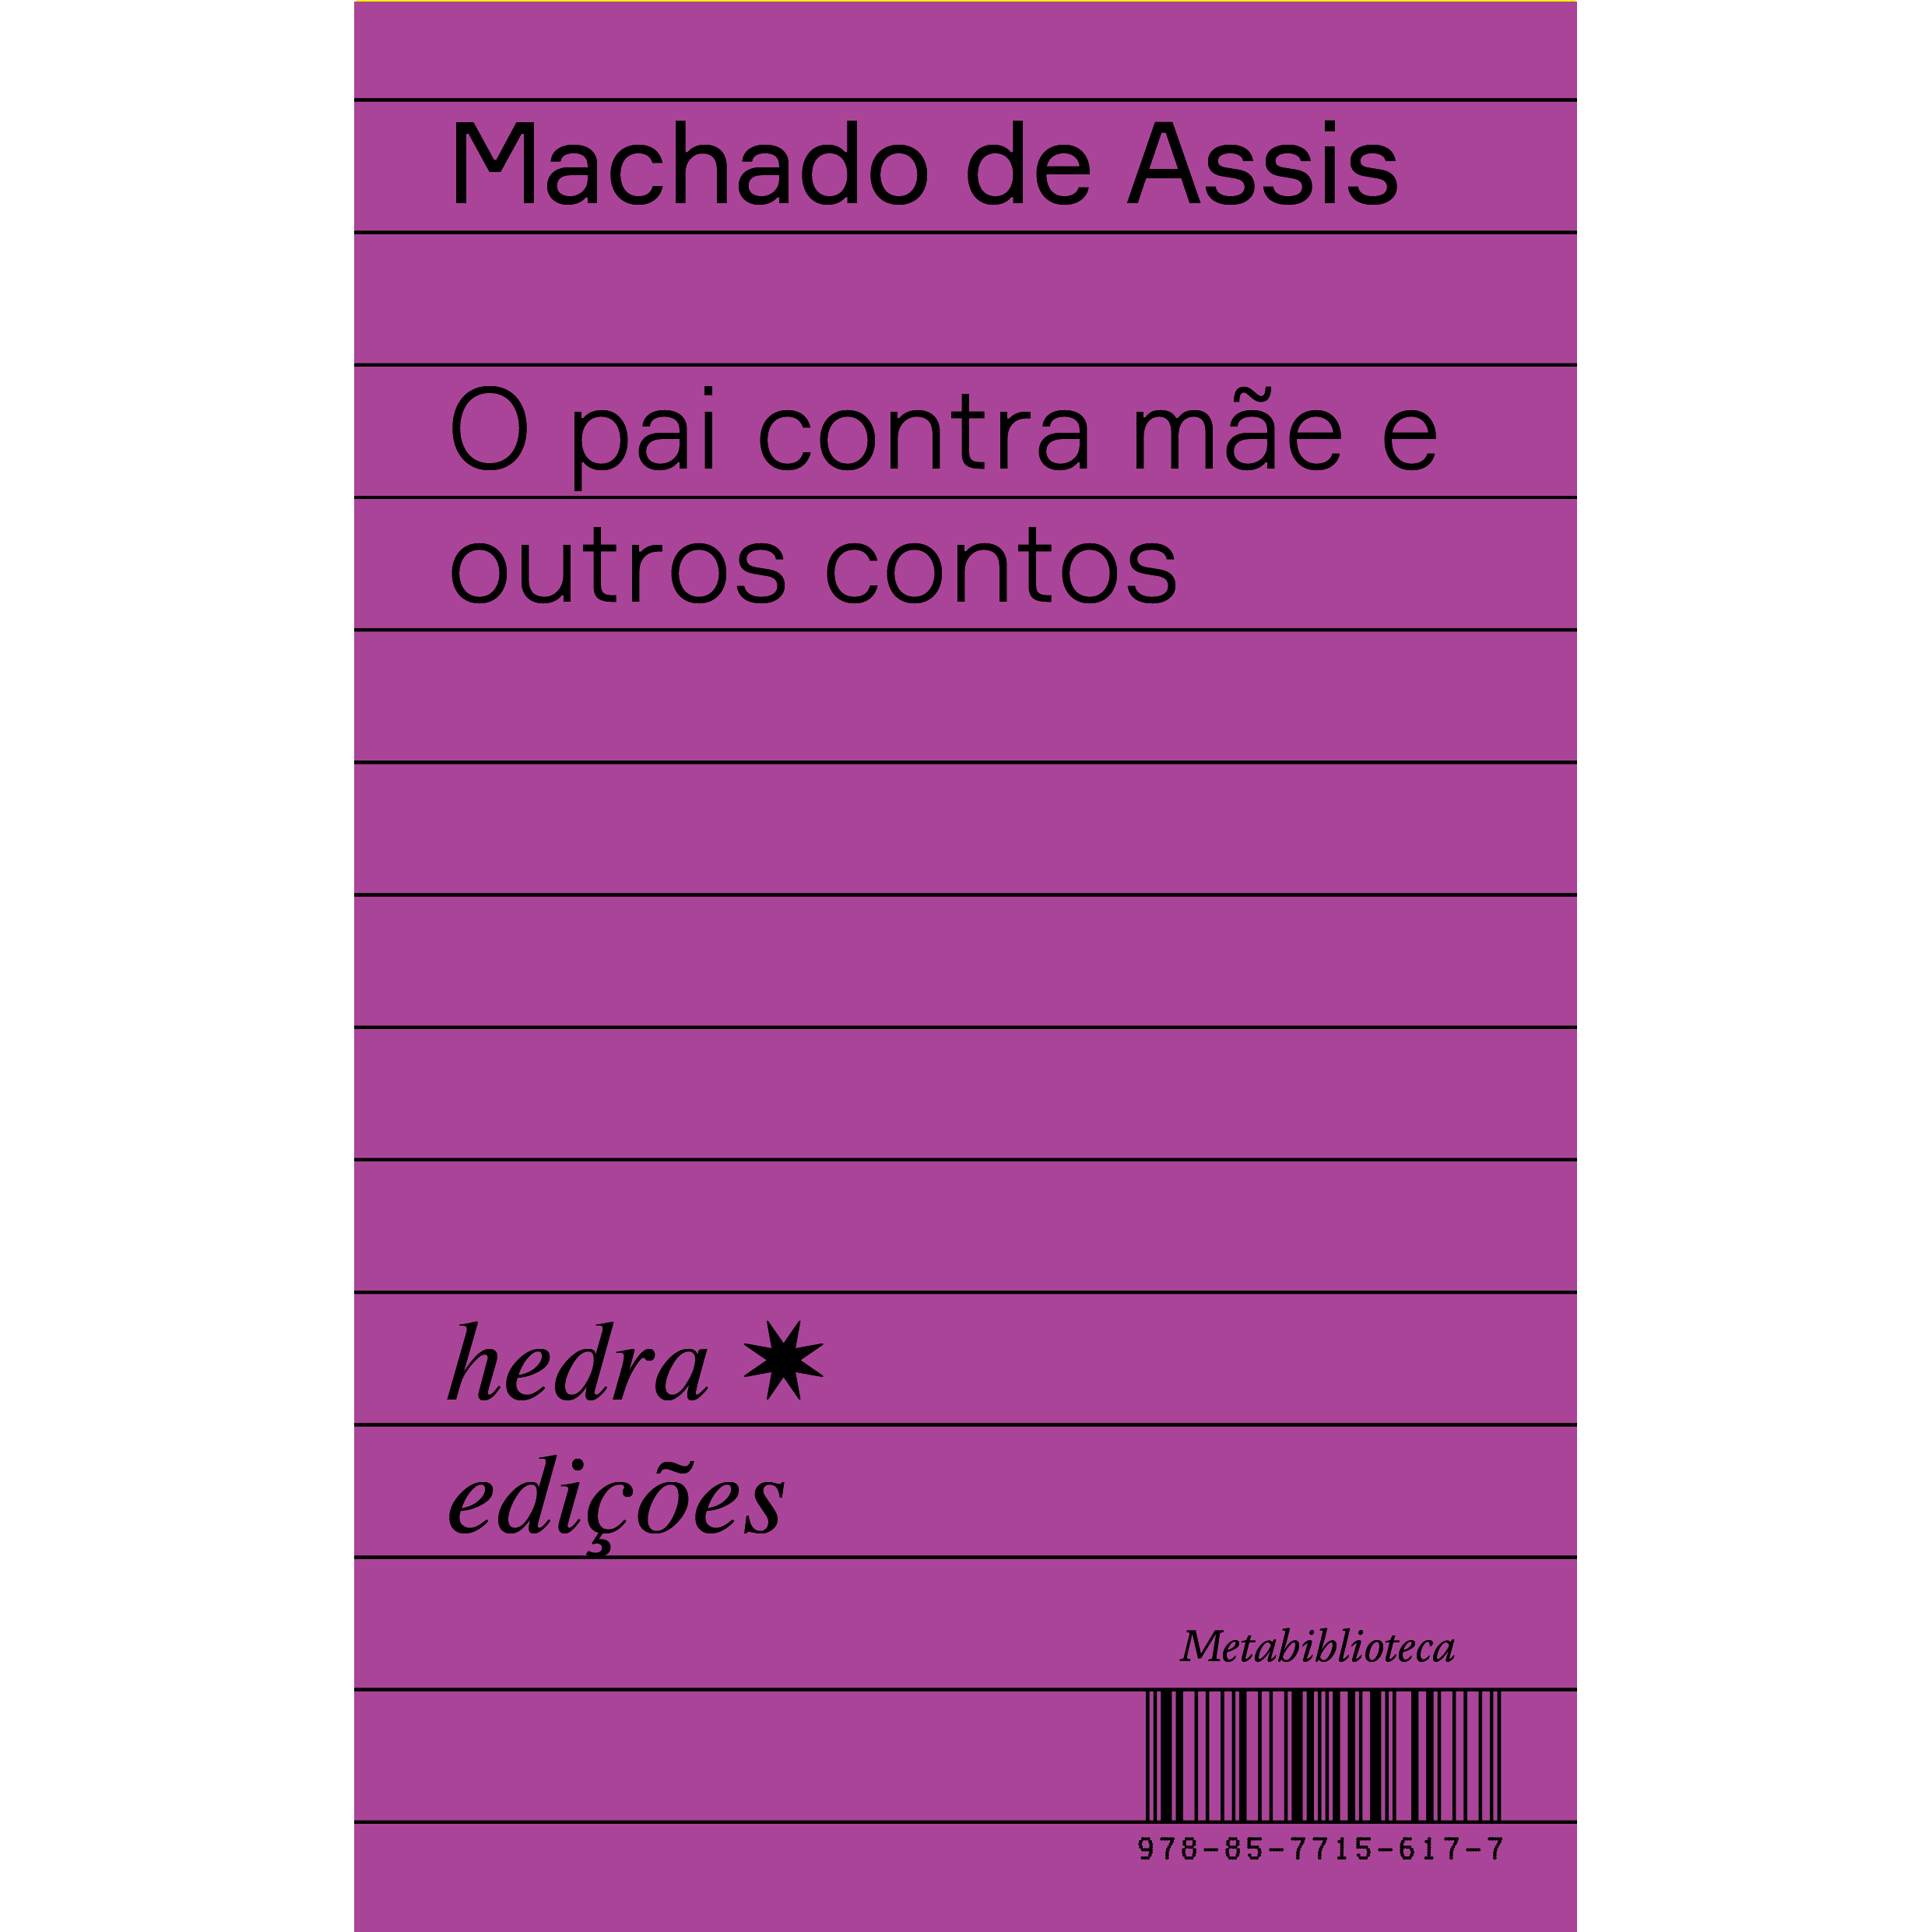
\includegraphics[width=46mm]{./grid/machado.jpg}}
\subfloat{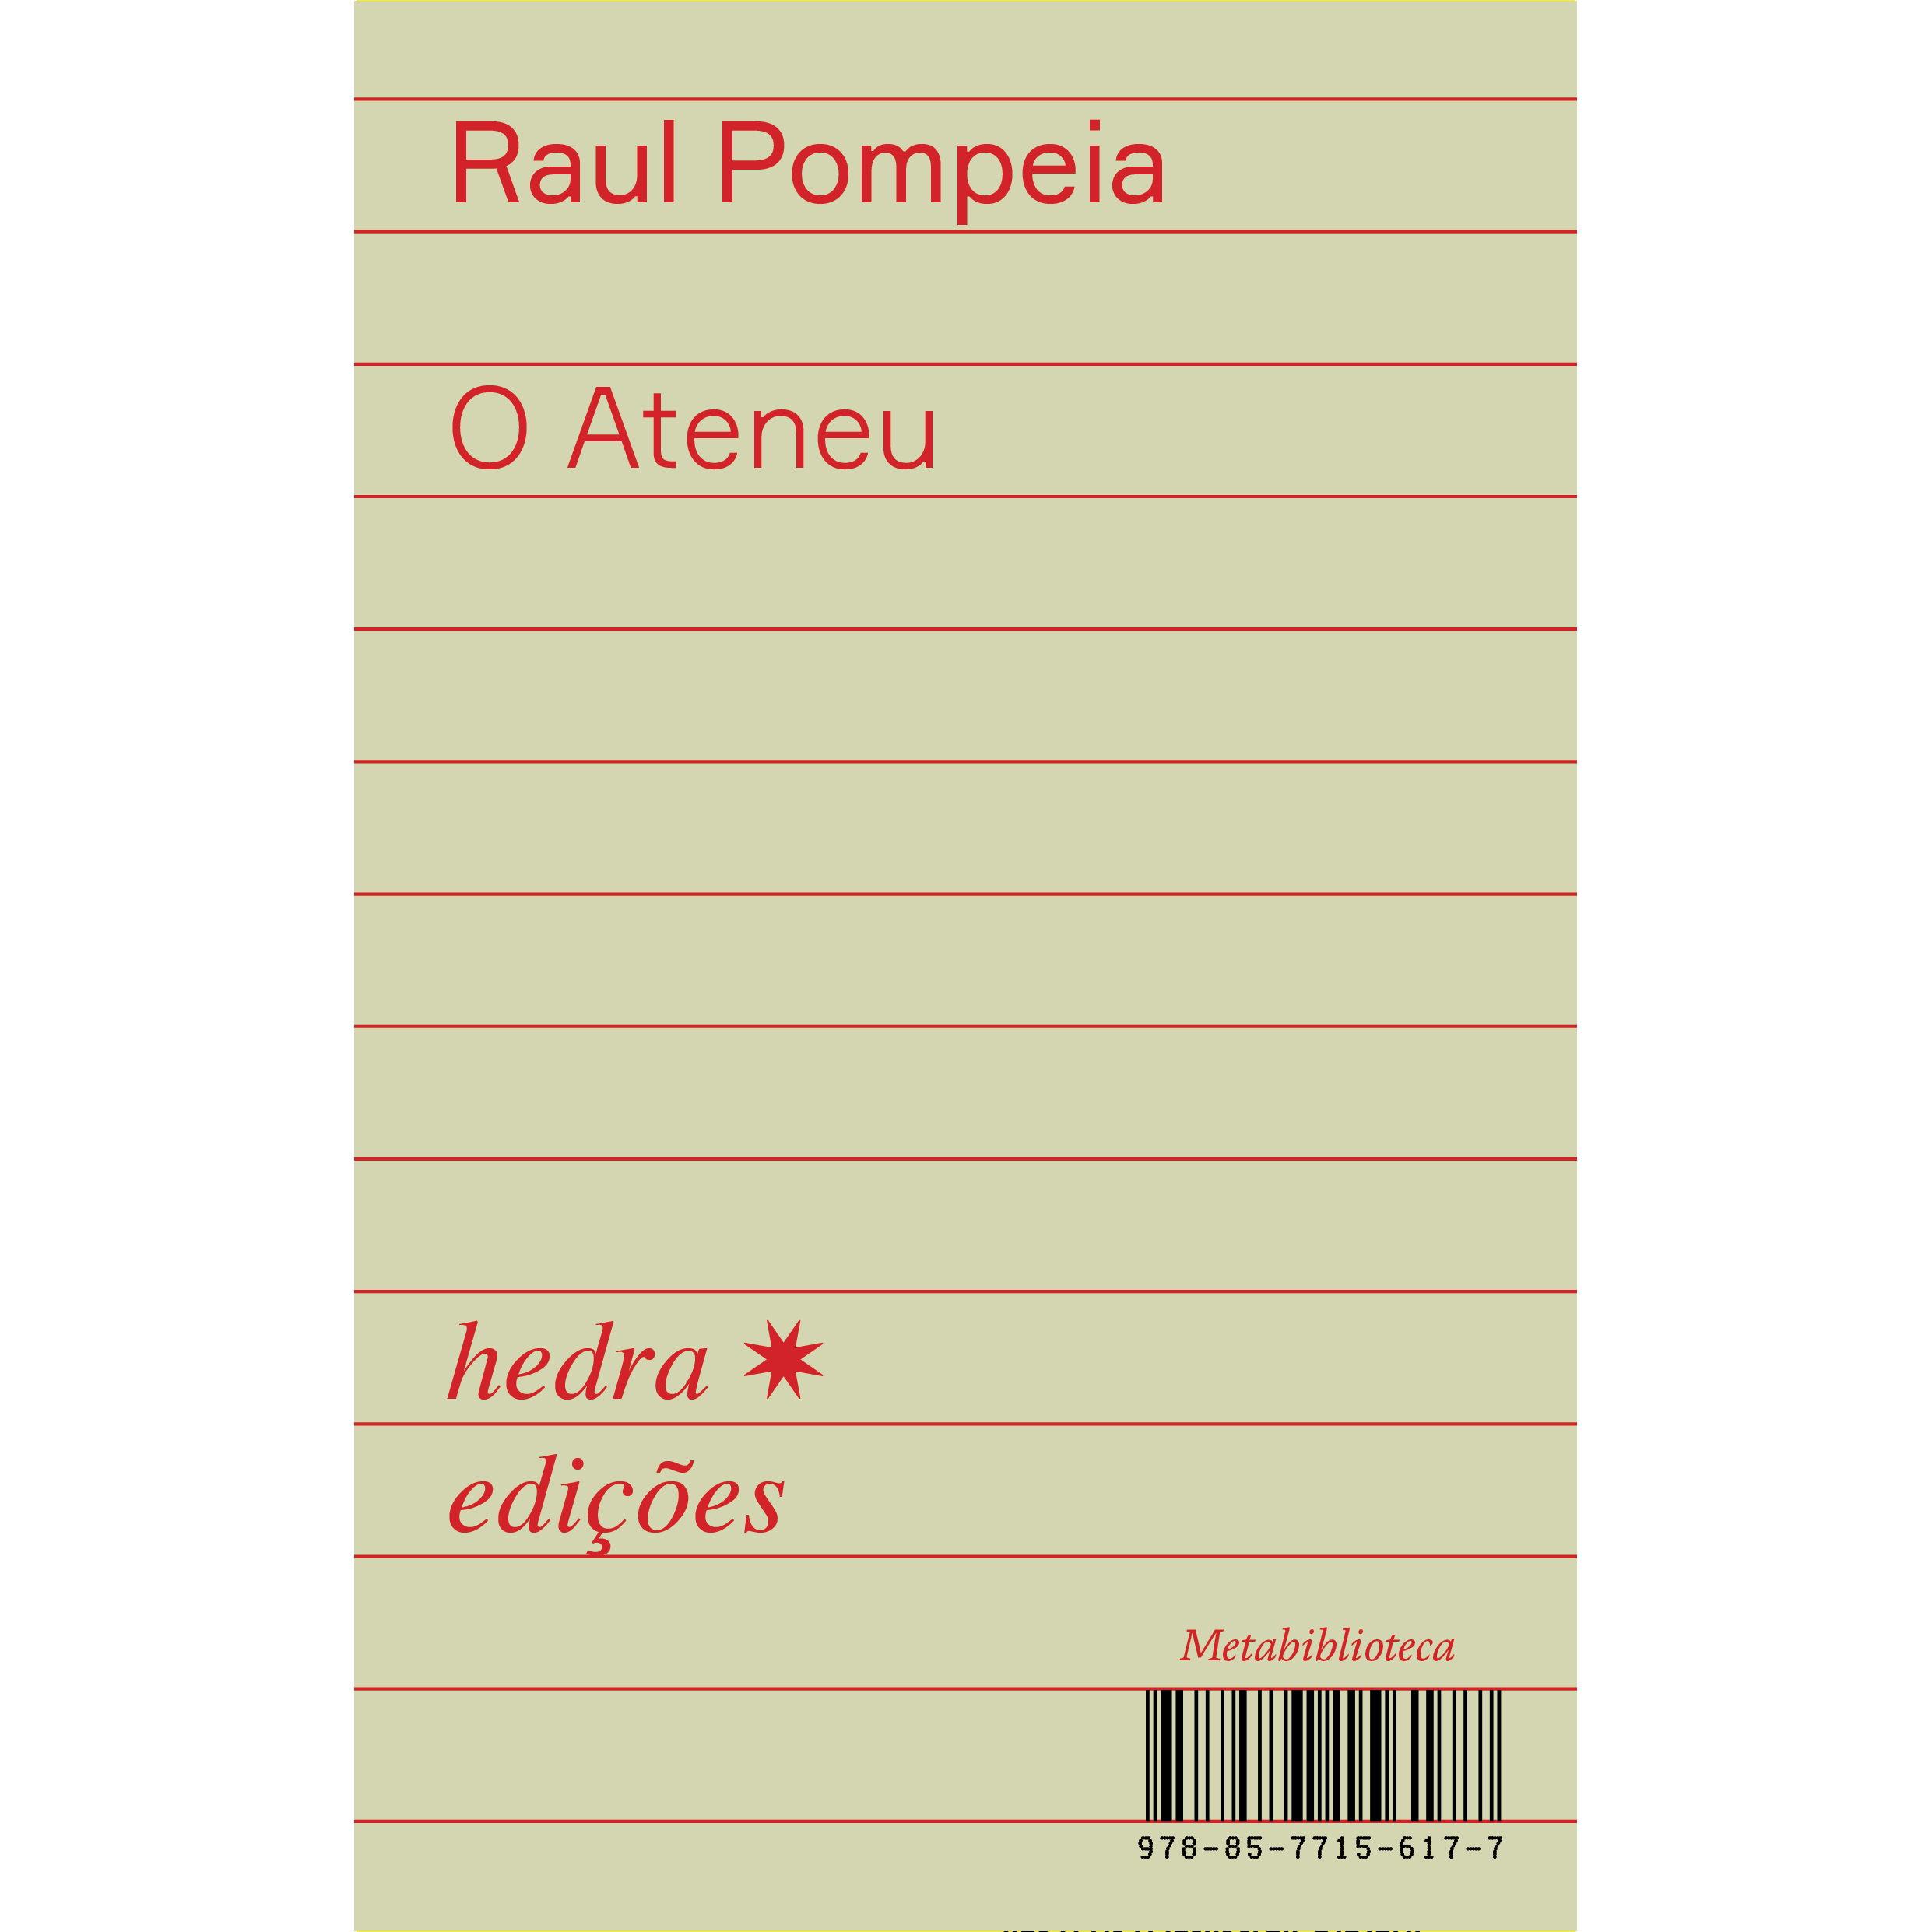
\includegraphics[width=46mm]{./grid/ateneu.jpg}}\\\hspace*{-.5cm}
\vspace{.5cm}
\subfloat{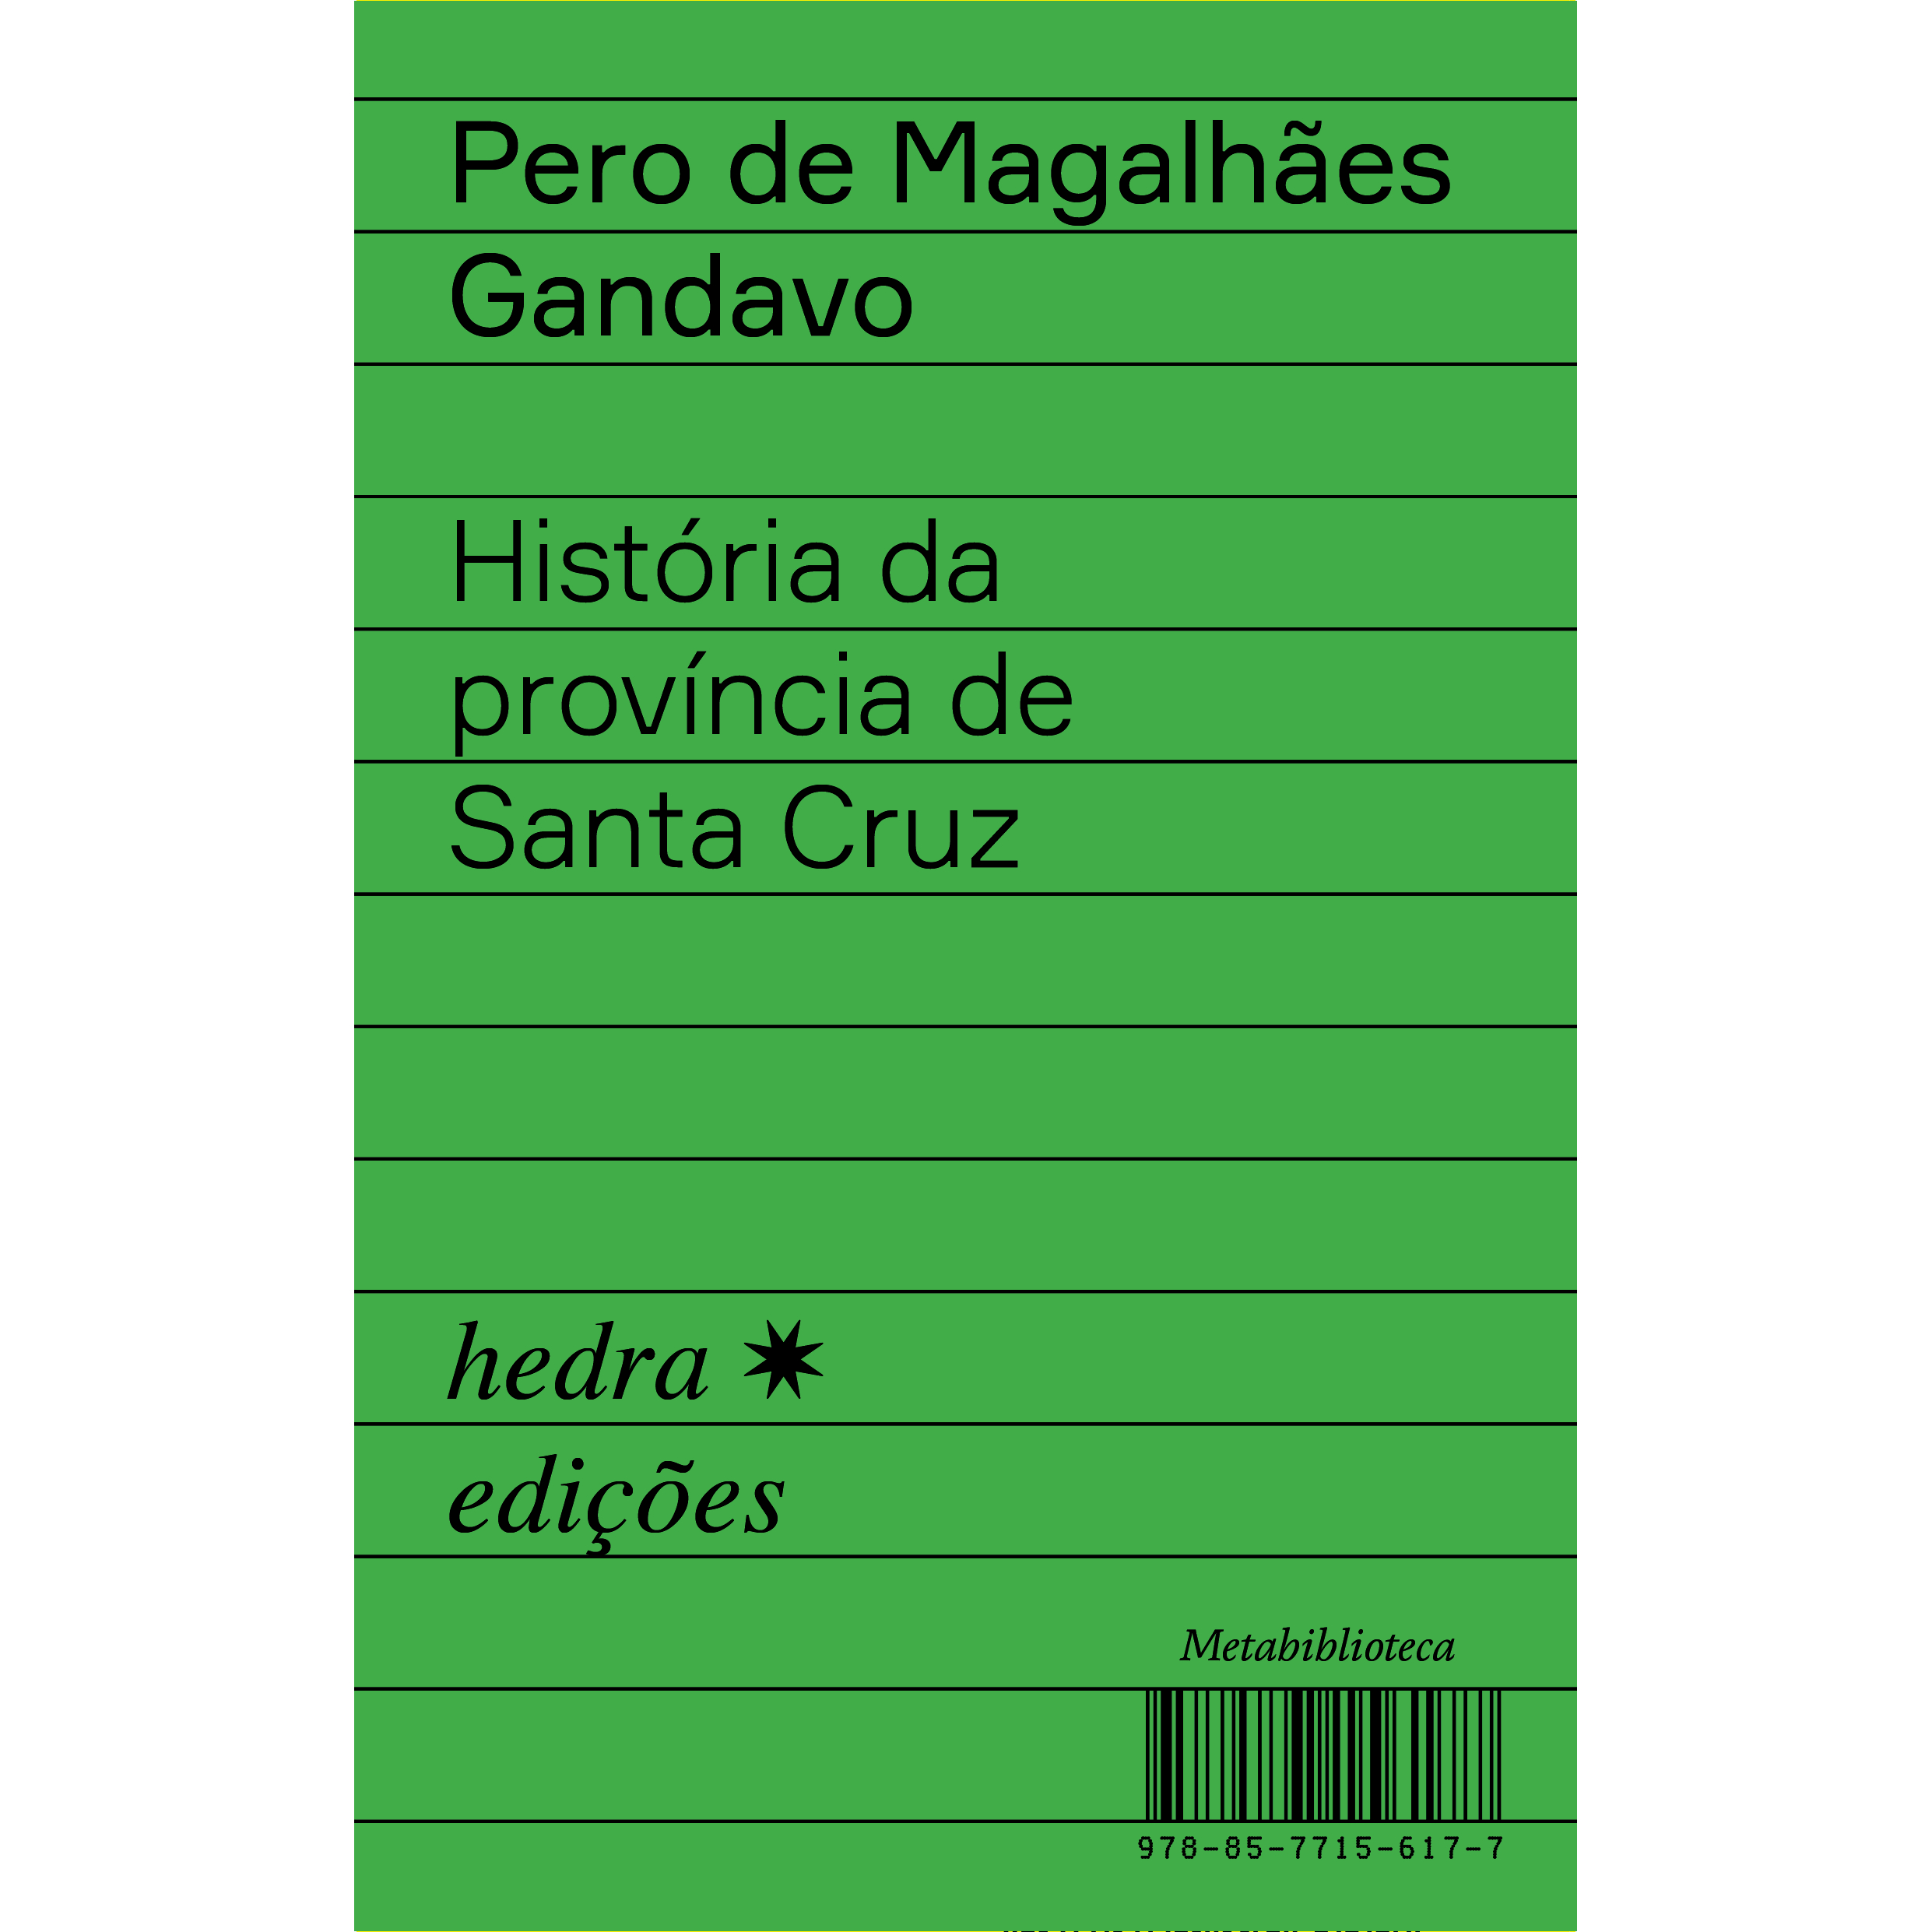
\includegraphics[width=46mm]{./grid/gandavo.jpg}}
\subfloat{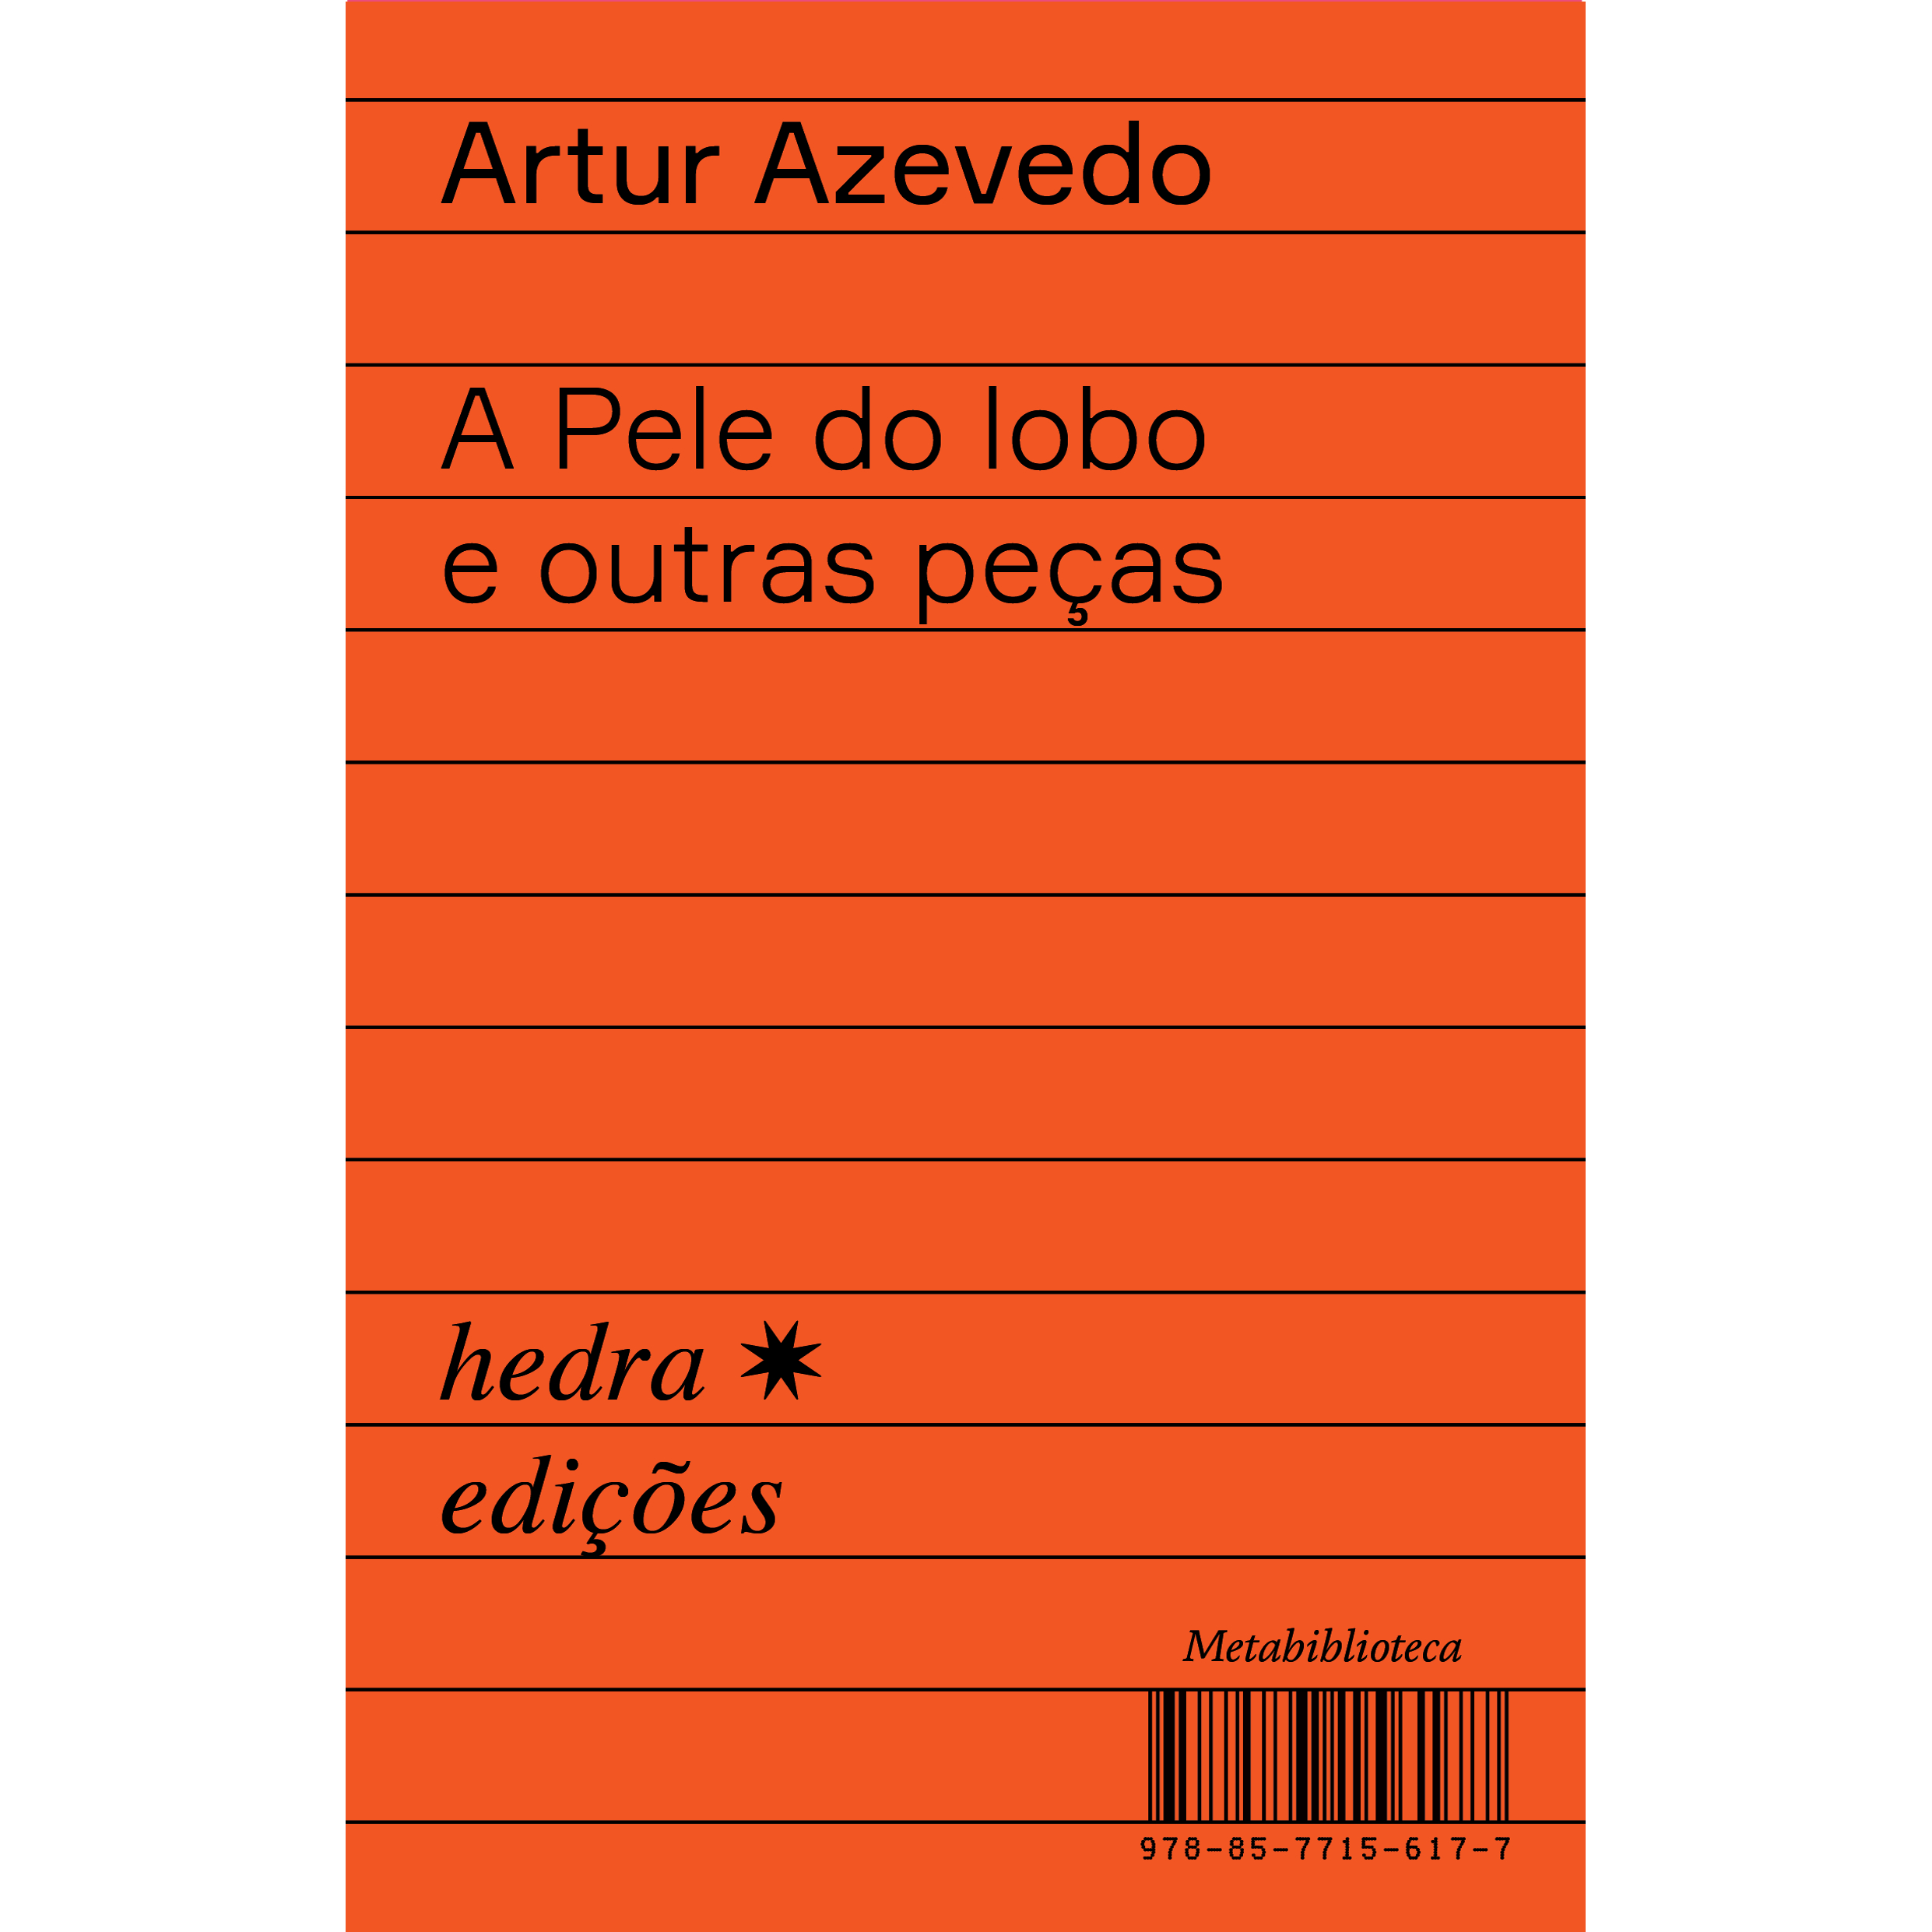
\includegraphics[width=46mm]{./grid/azevedo.jpg}}
\subfloat{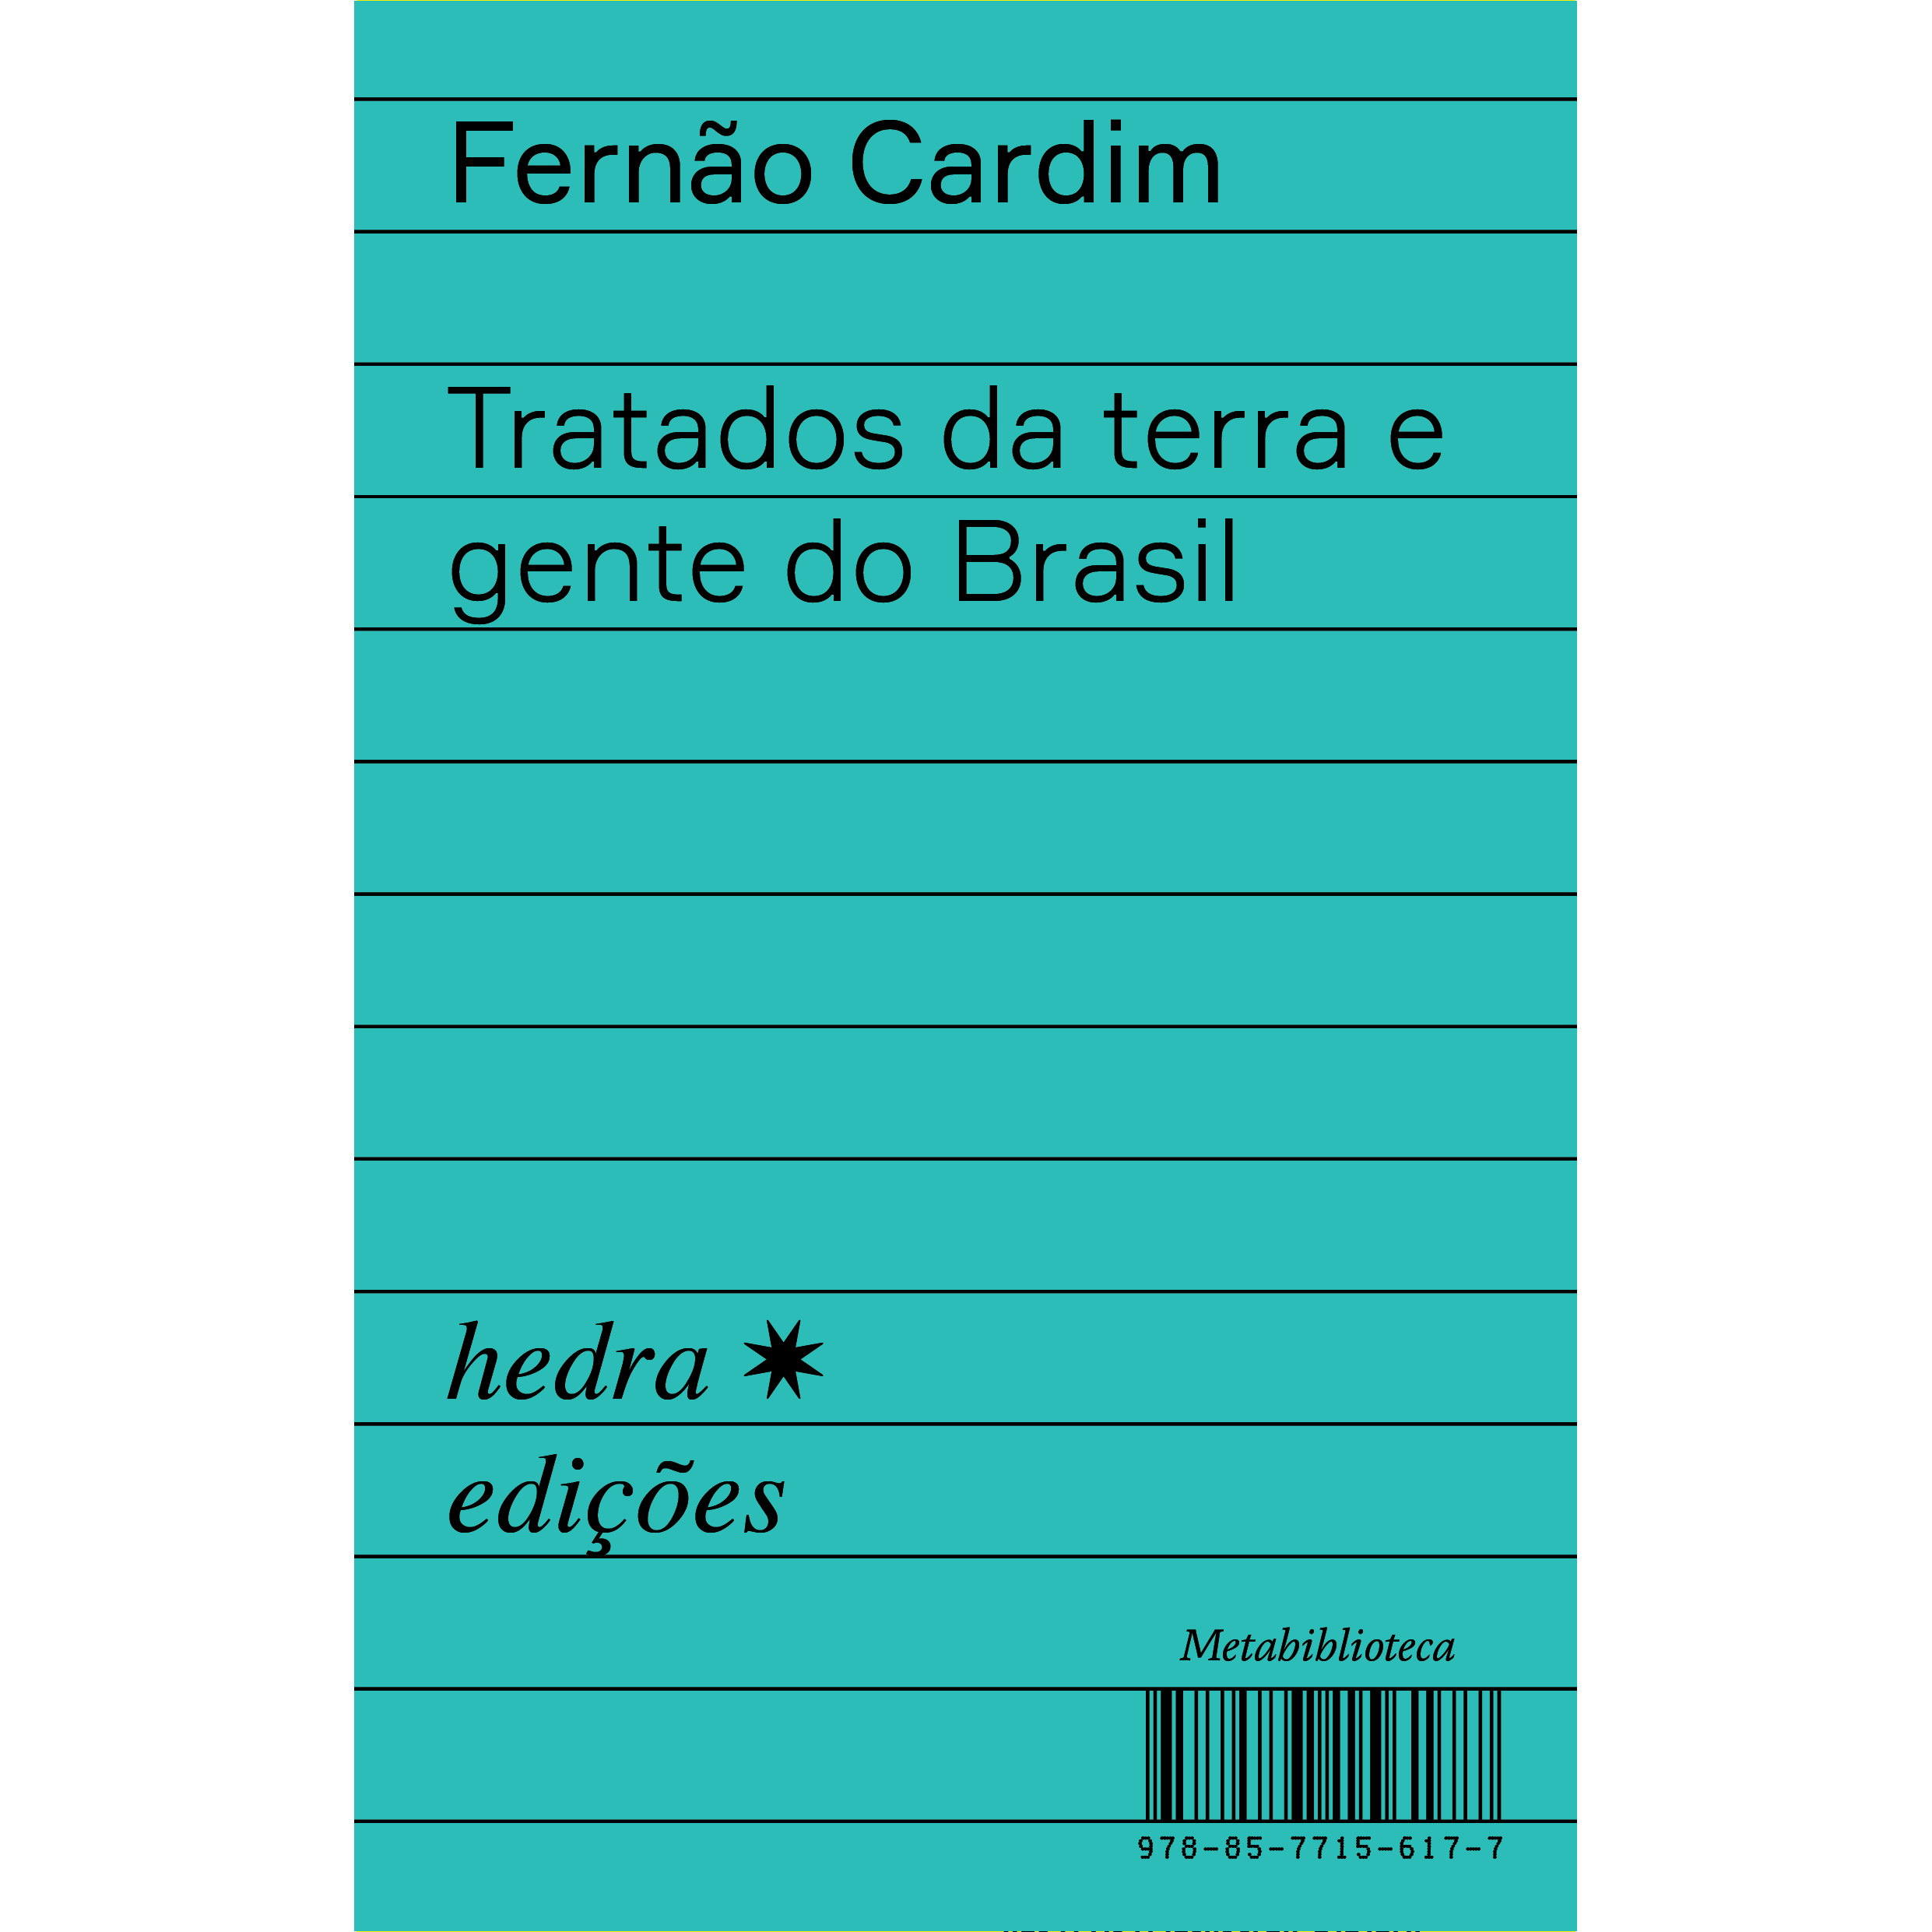
\includegraphics[width=46mm]{./grid/cardim.jpg}}\\\hspace*{-.5cm}
\vspace{.5cm}
\subfloat{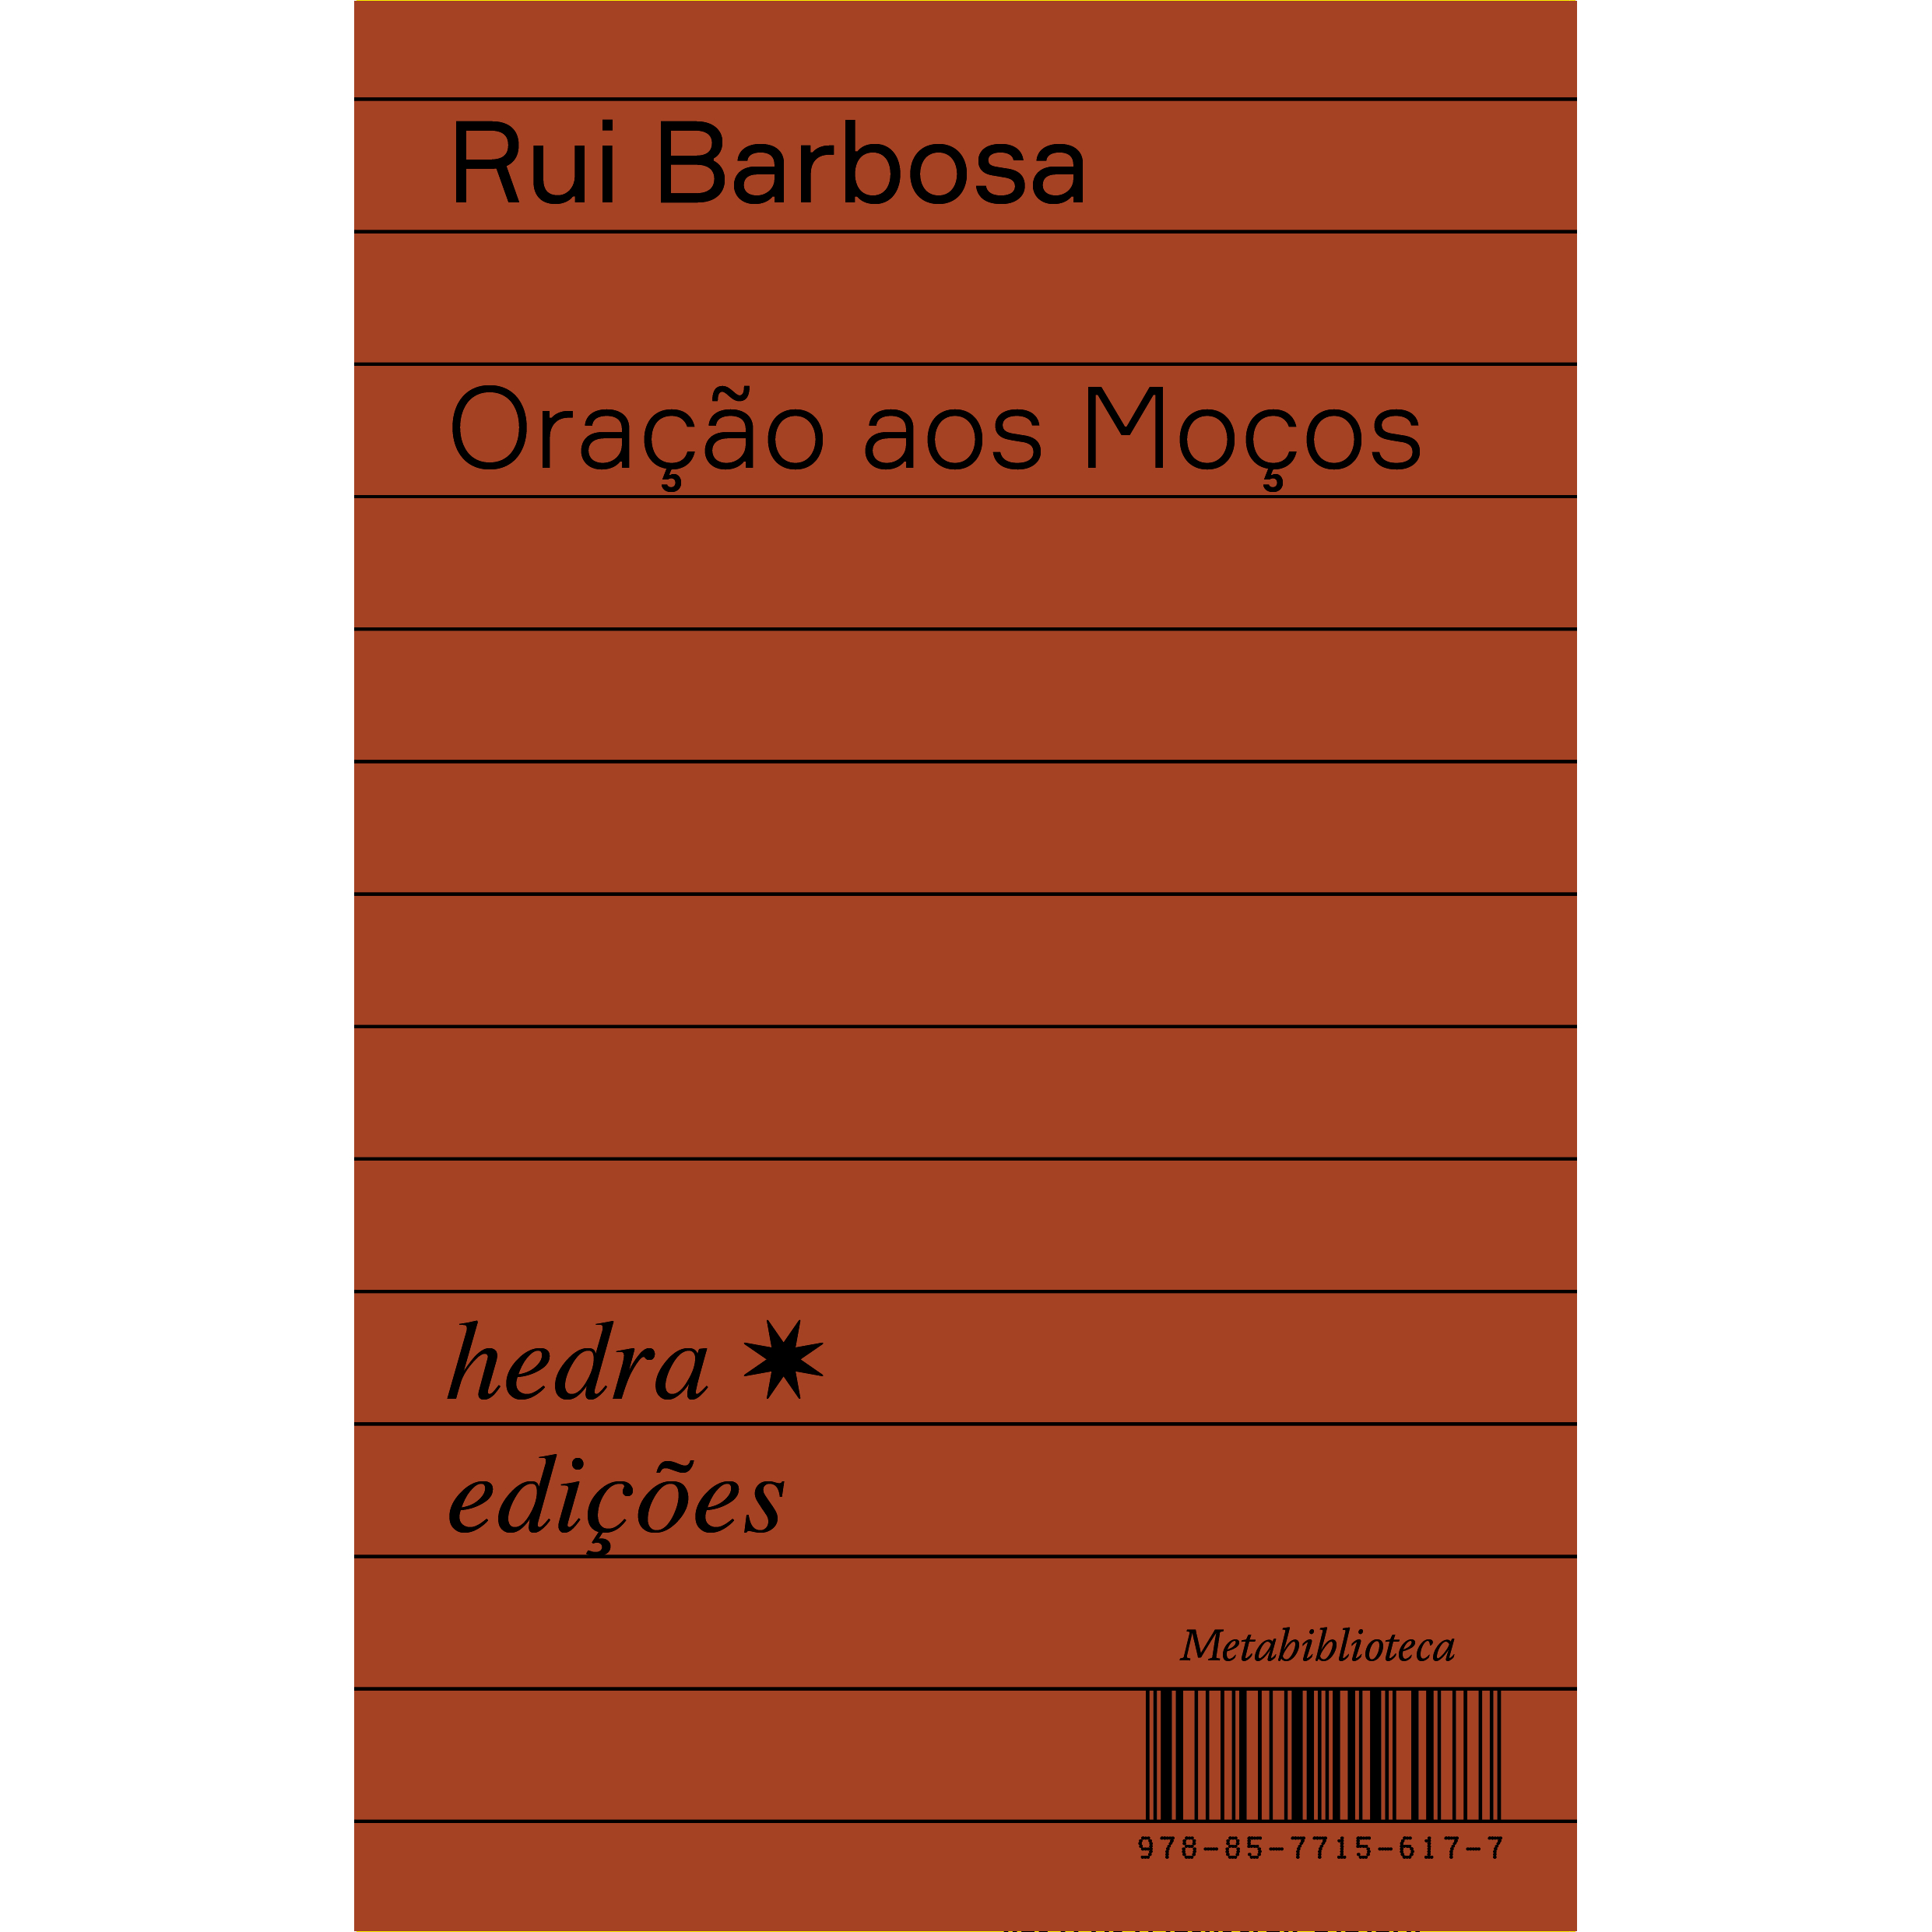
\includegraphics[width=46mm]{./grid/barbosa.jpg}}
\subfloat{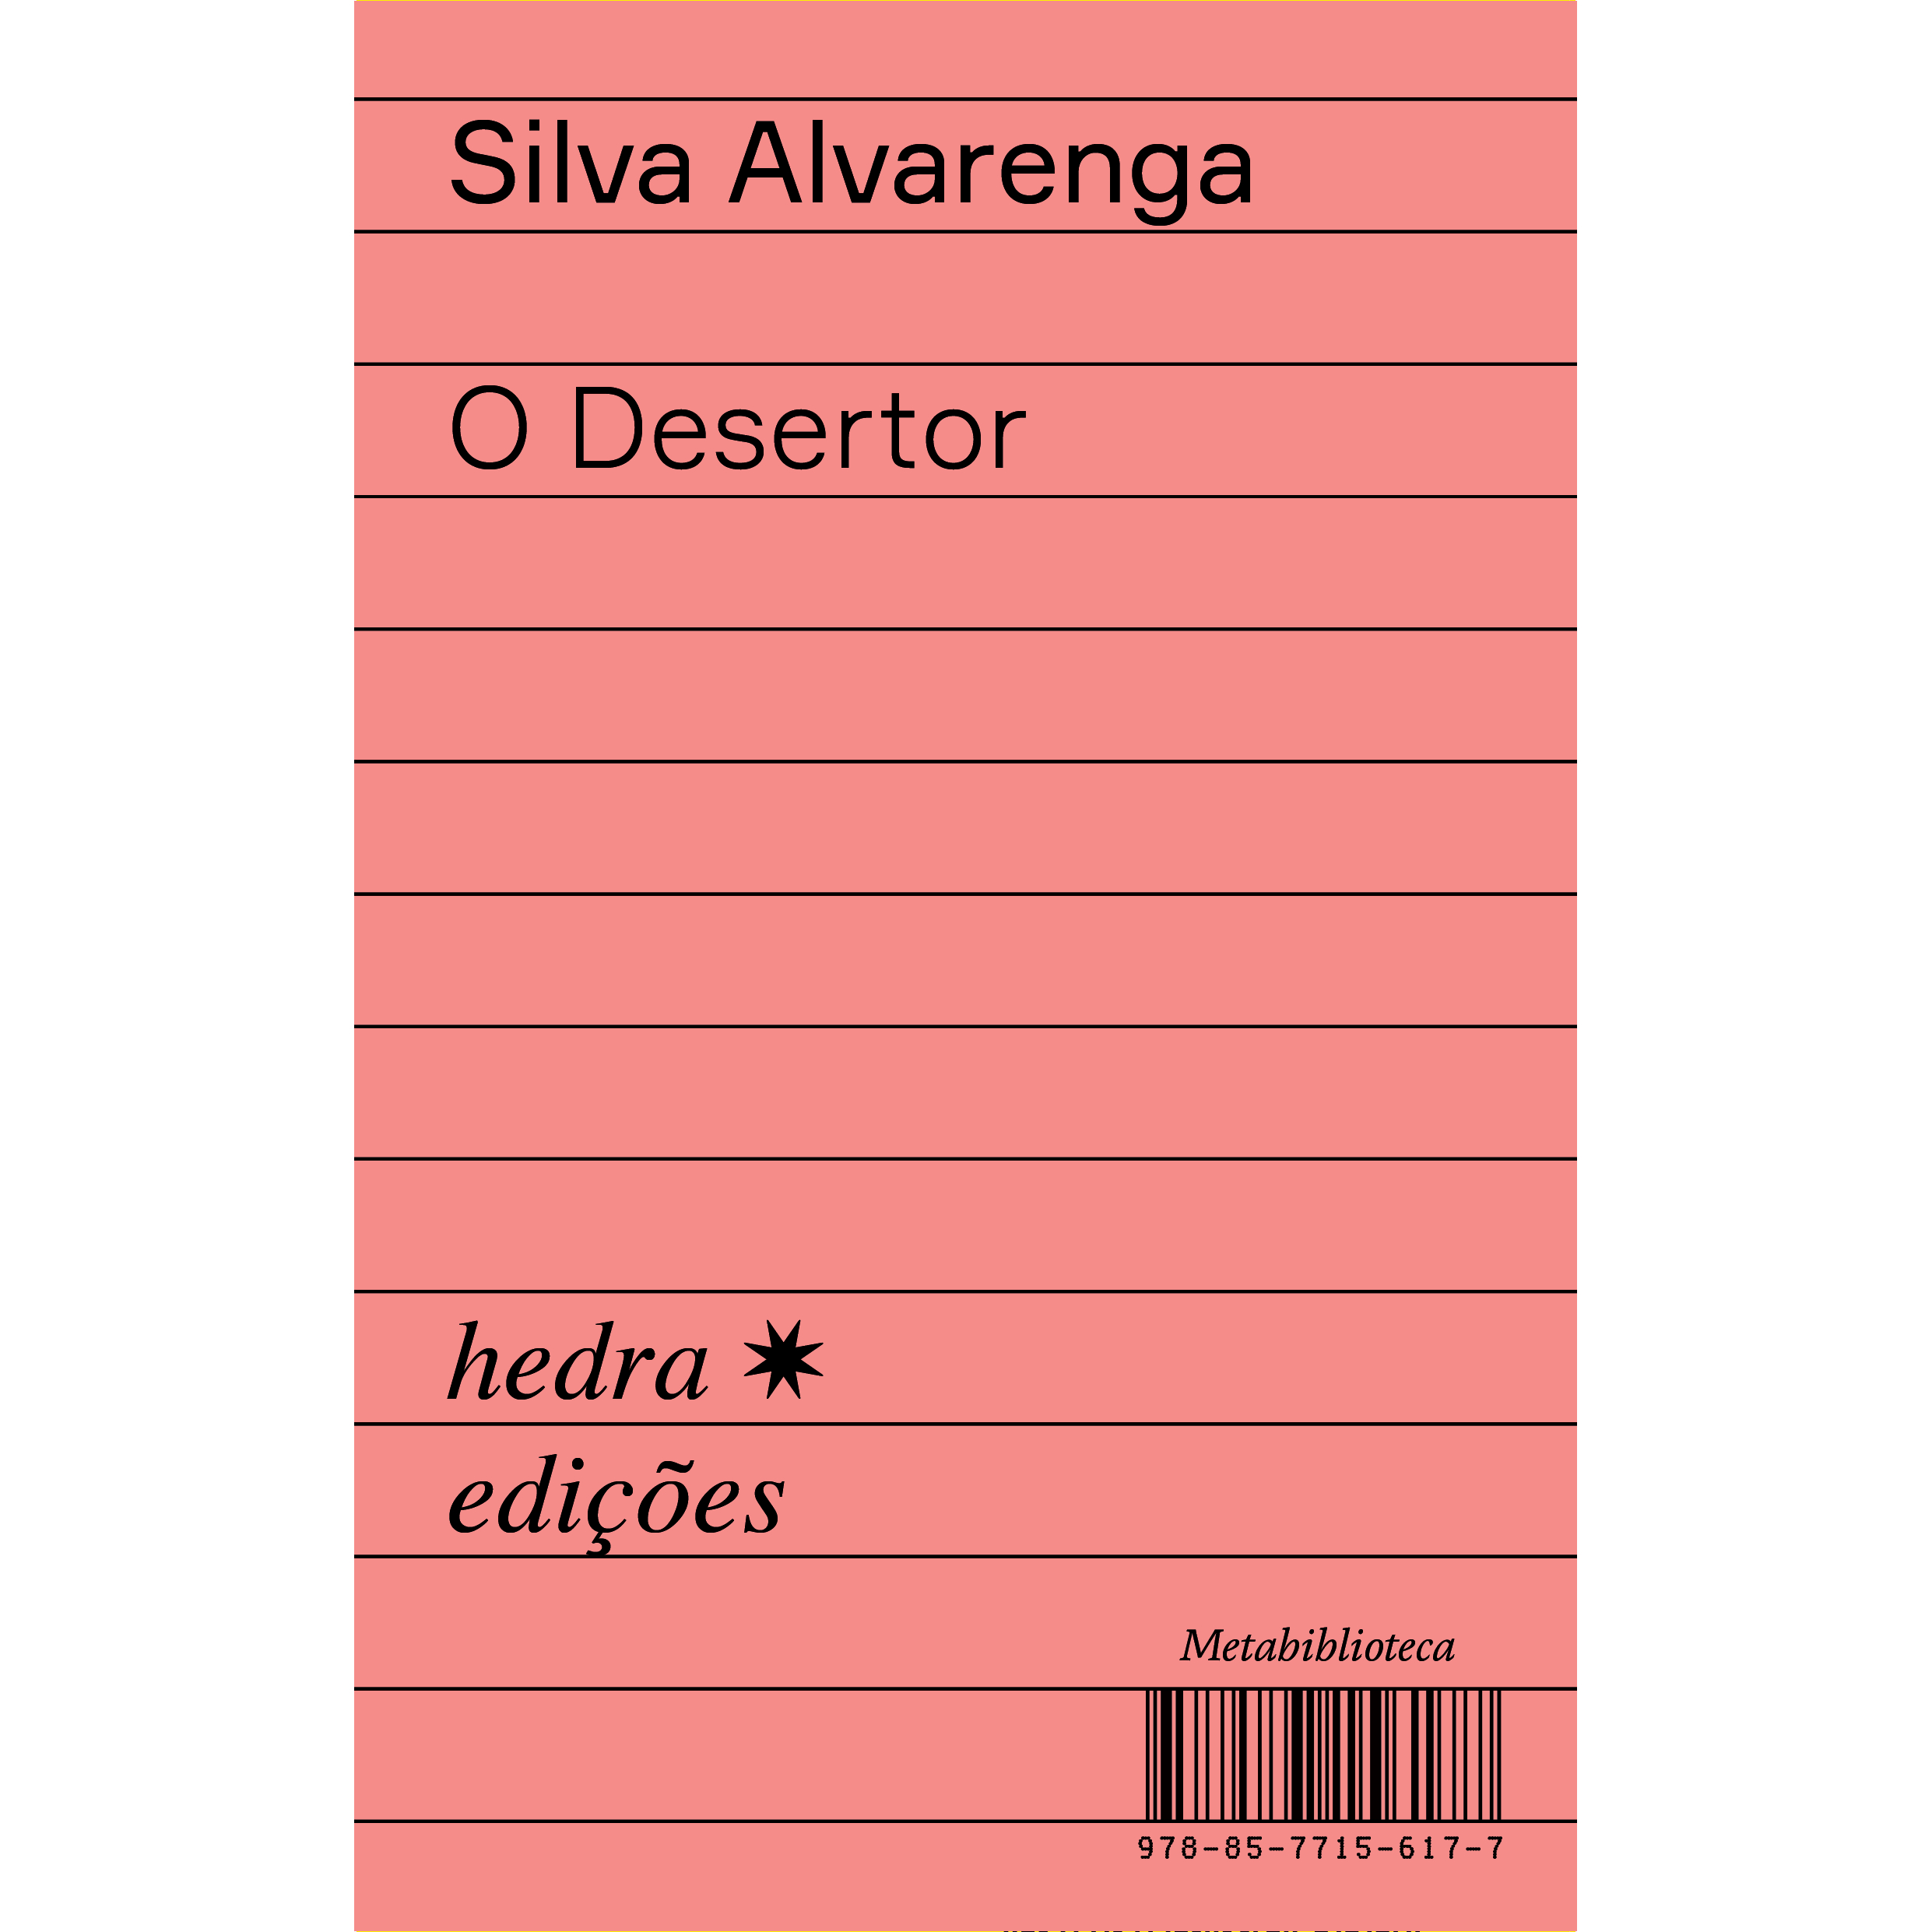
\includegraphics[width=46mm]{./grid/desertor.jpg}}
\subfloat{
\includegraphics[width=46mm]{./grid/tratado.jpg}}\\\hspace*{-.5cm}
\vspace{.5cm}
\subfloat{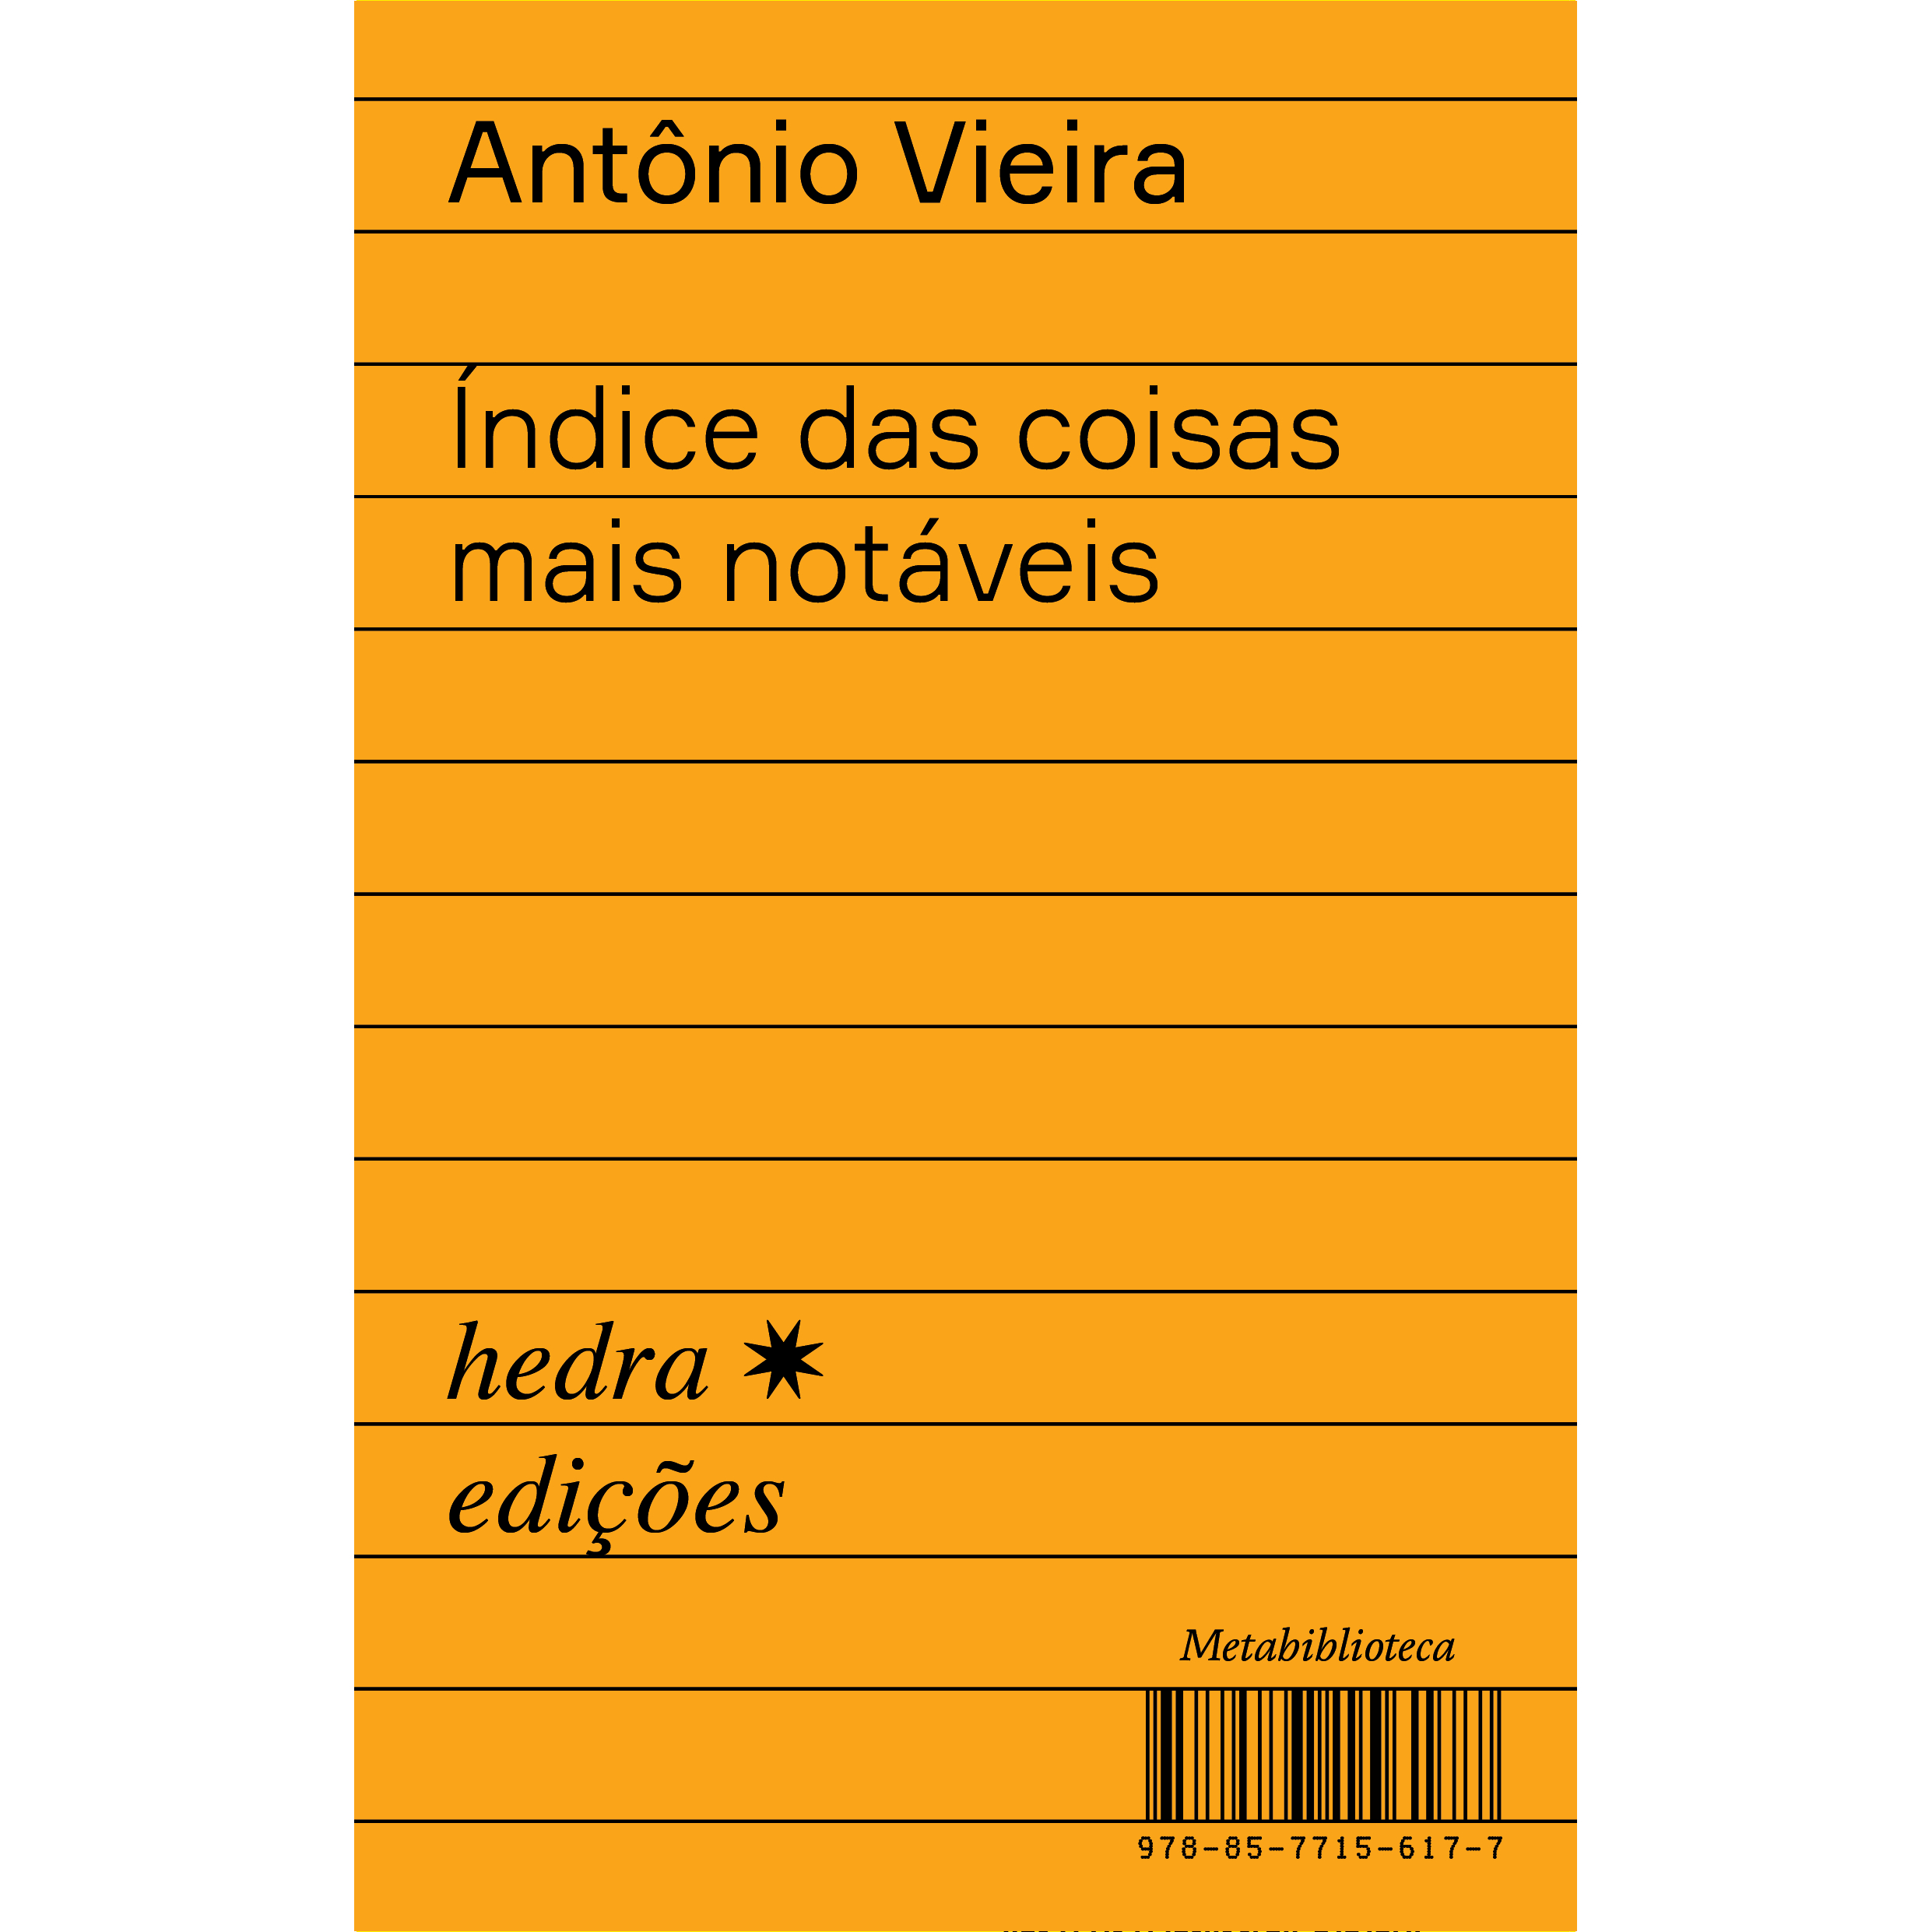
\includegraphics[width=46mm]{./grid/vieira.jpg}}
\subfloat{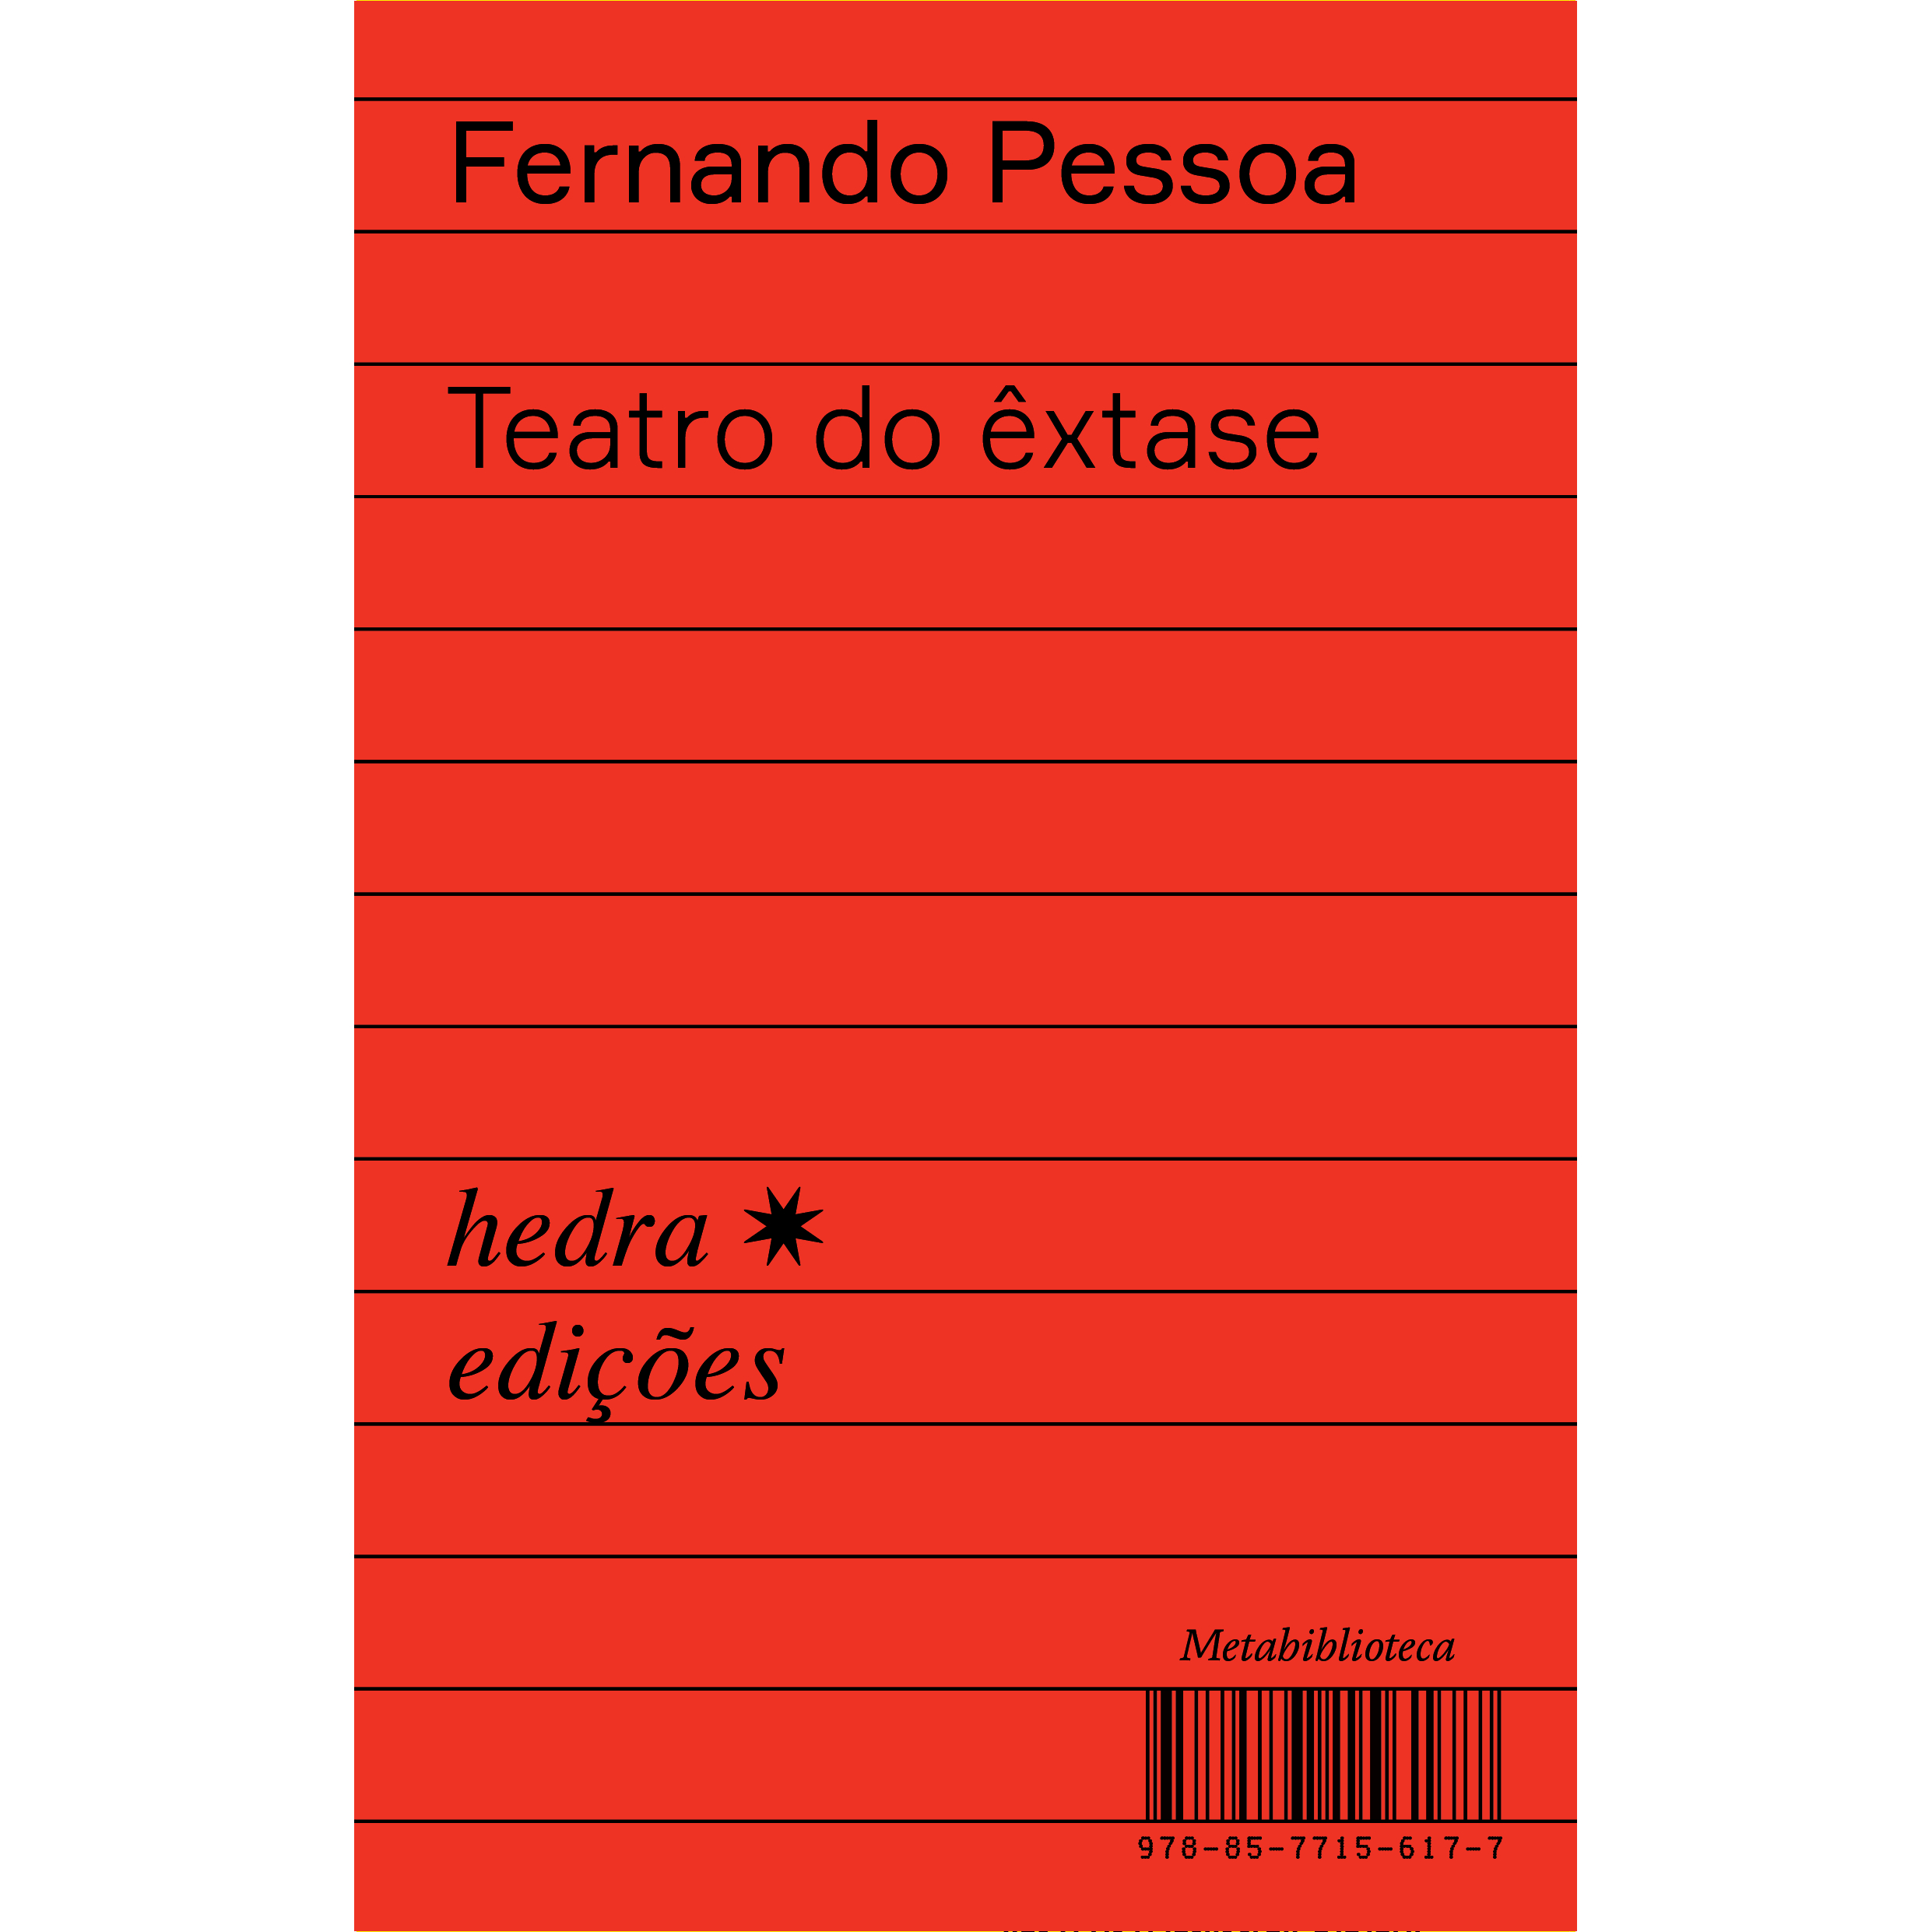
\includegraphics[width=46mm]{./grid/pessoa.jpg}}
\subfloat{
\includegraphics[width=46mm]{./grid/benjamin.jpg}}\\
\end{tabular}
\end{figure}

\pagebreak

\begin{figure}[!htbp]
\begin{tabular}{cccc}

\vspace{.5cm}
\hspace*{-.5cm}
\subfloat{
\includegraphics[width=46mm]{./grid/benjamin2.jpg}}
\subfloat{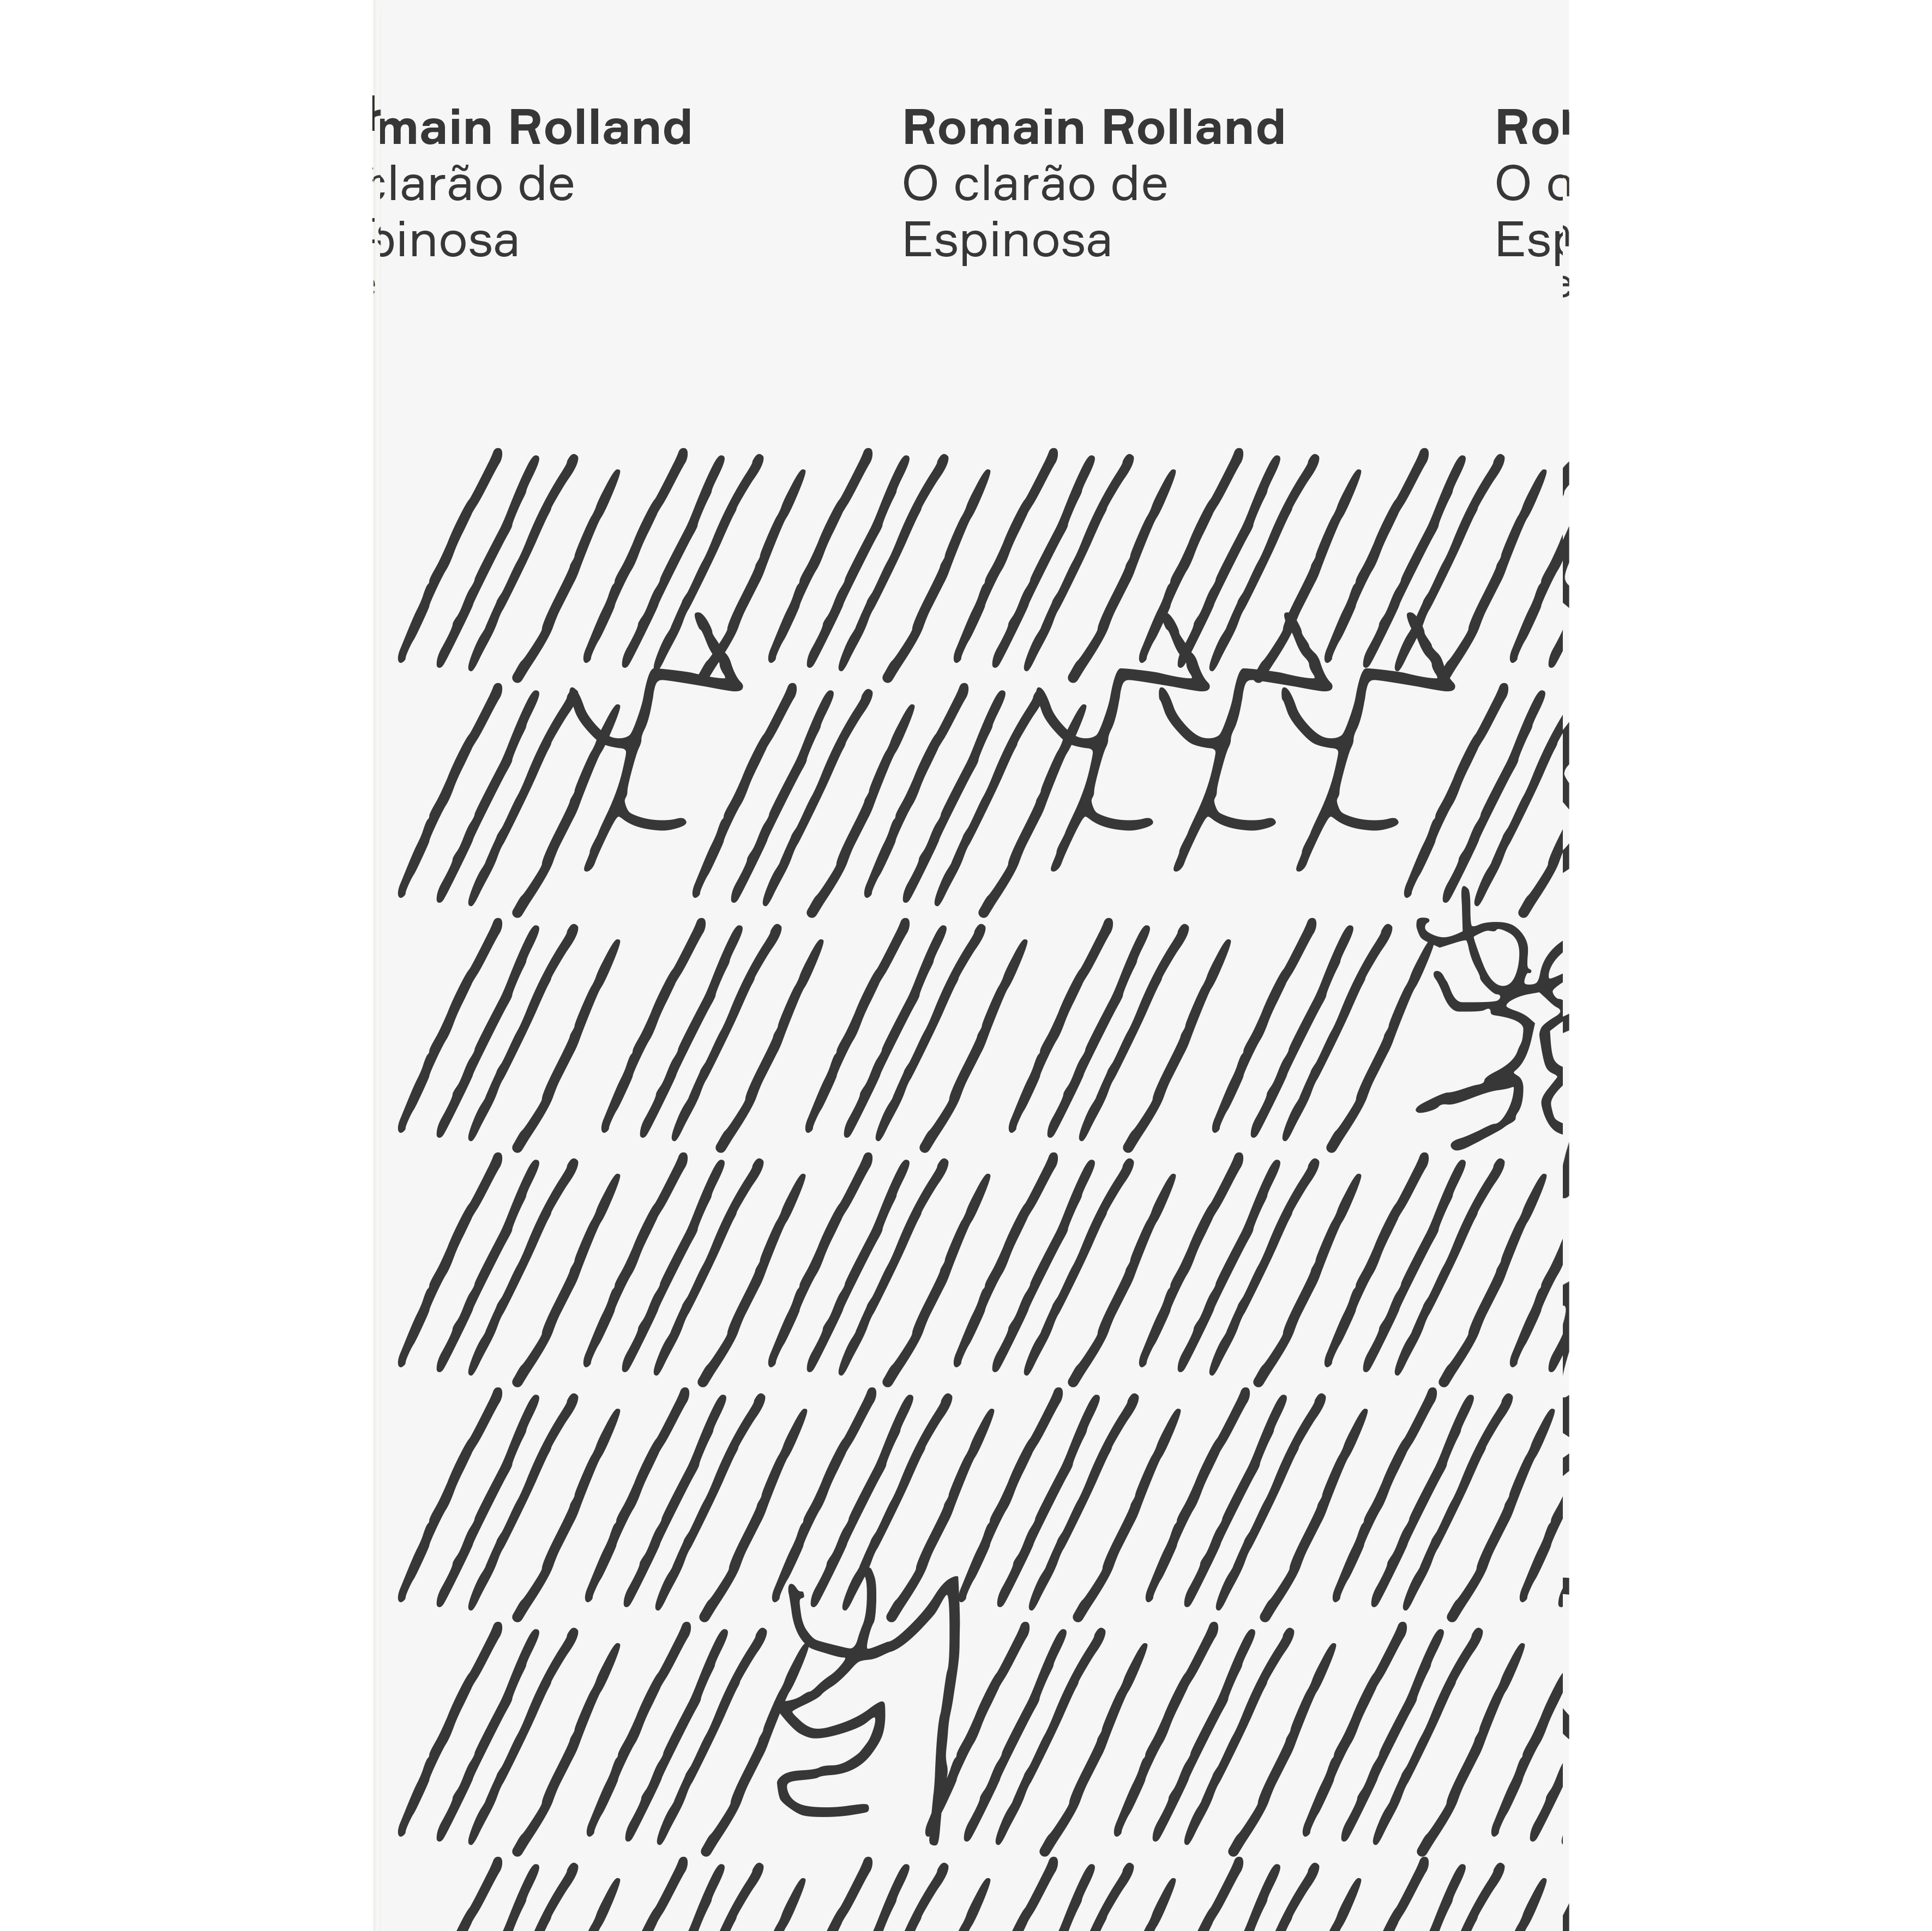
\includegraphics[width=46mm]{./grid/rolland.png}}
\subfloat{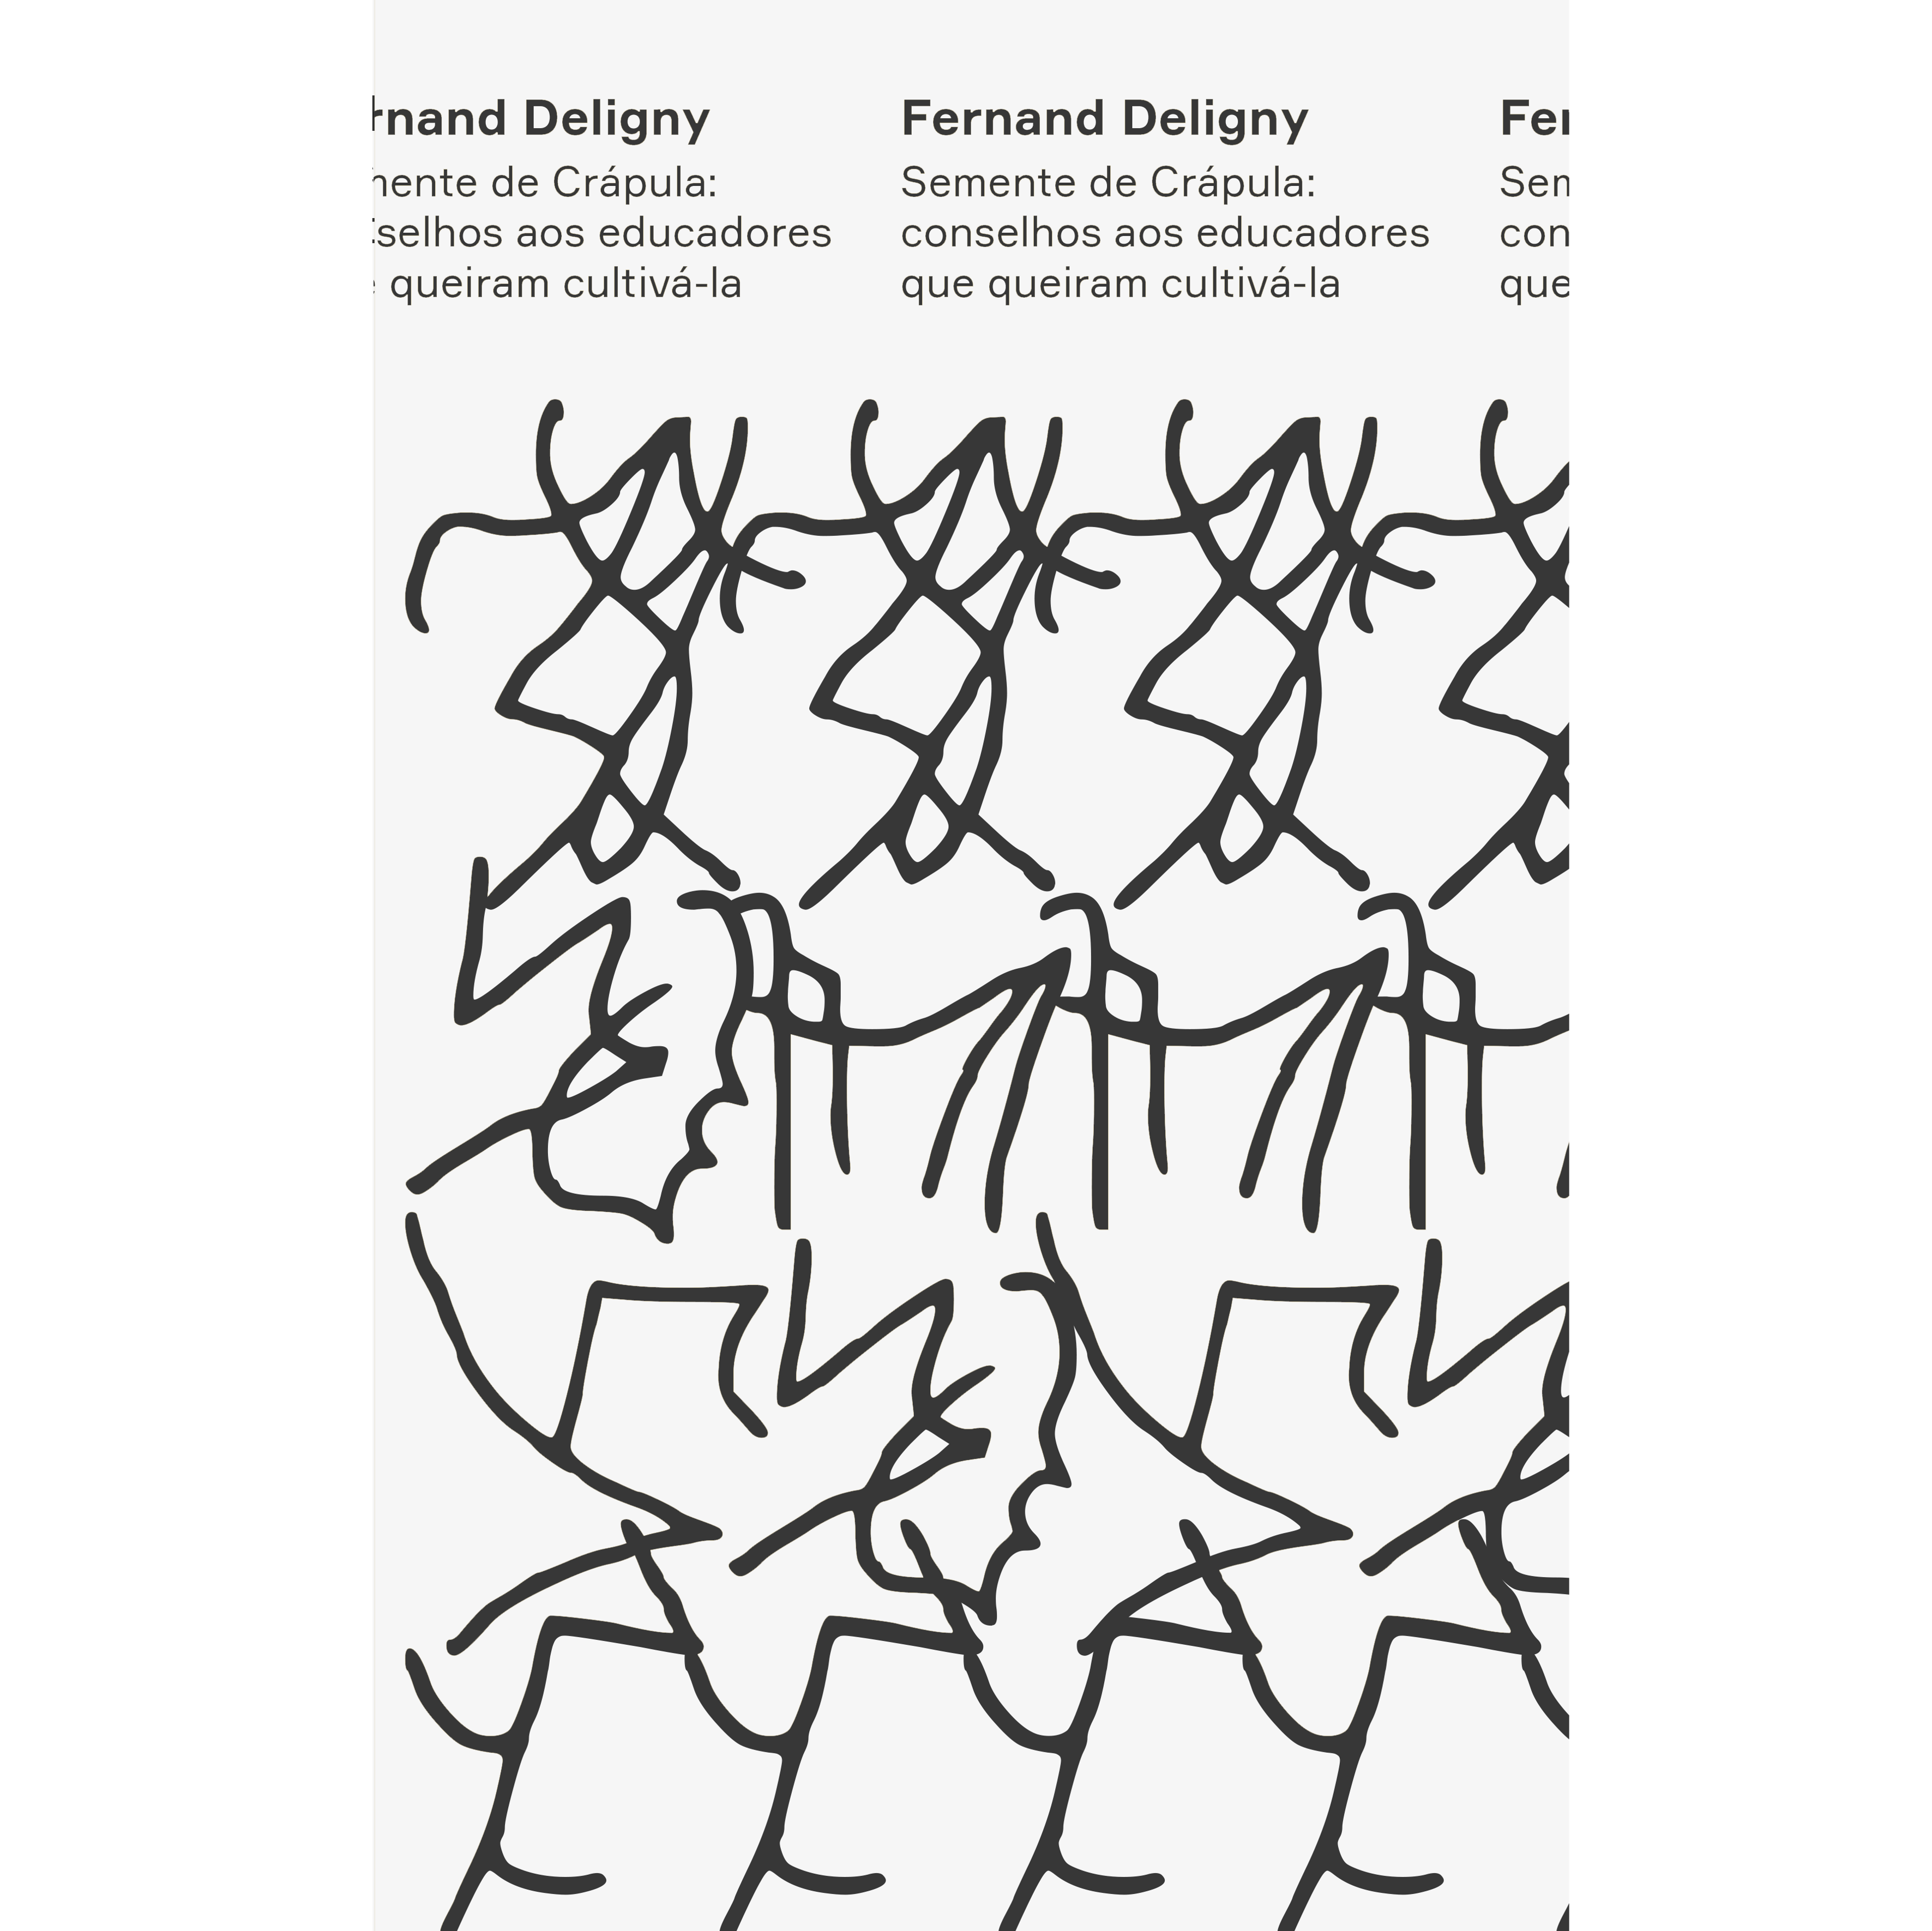
\includegraphics[width=46mm]{./grid/deligny.png}}\\\hspace*{-.5cm}
\vspace{.5cm}
\subfloat{
\includegraphics[width=46mm]{./grid/lovecraft.jpg}}
\subfloat{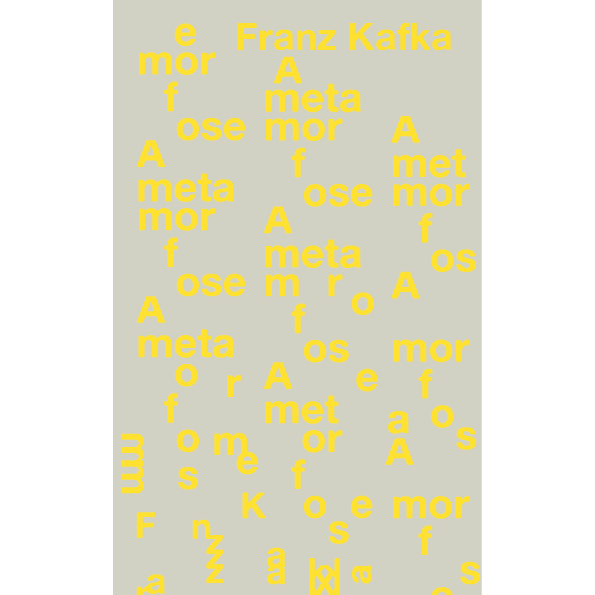
\includegraphics[width=46mm]{./grid/kafka.png}}
\subfloat{
\includegraphics[width=46mm]{./grid/maquiavel.jpg}}\\\hspace*{-.5cm}
\vspace{.5cm}
\subfloat{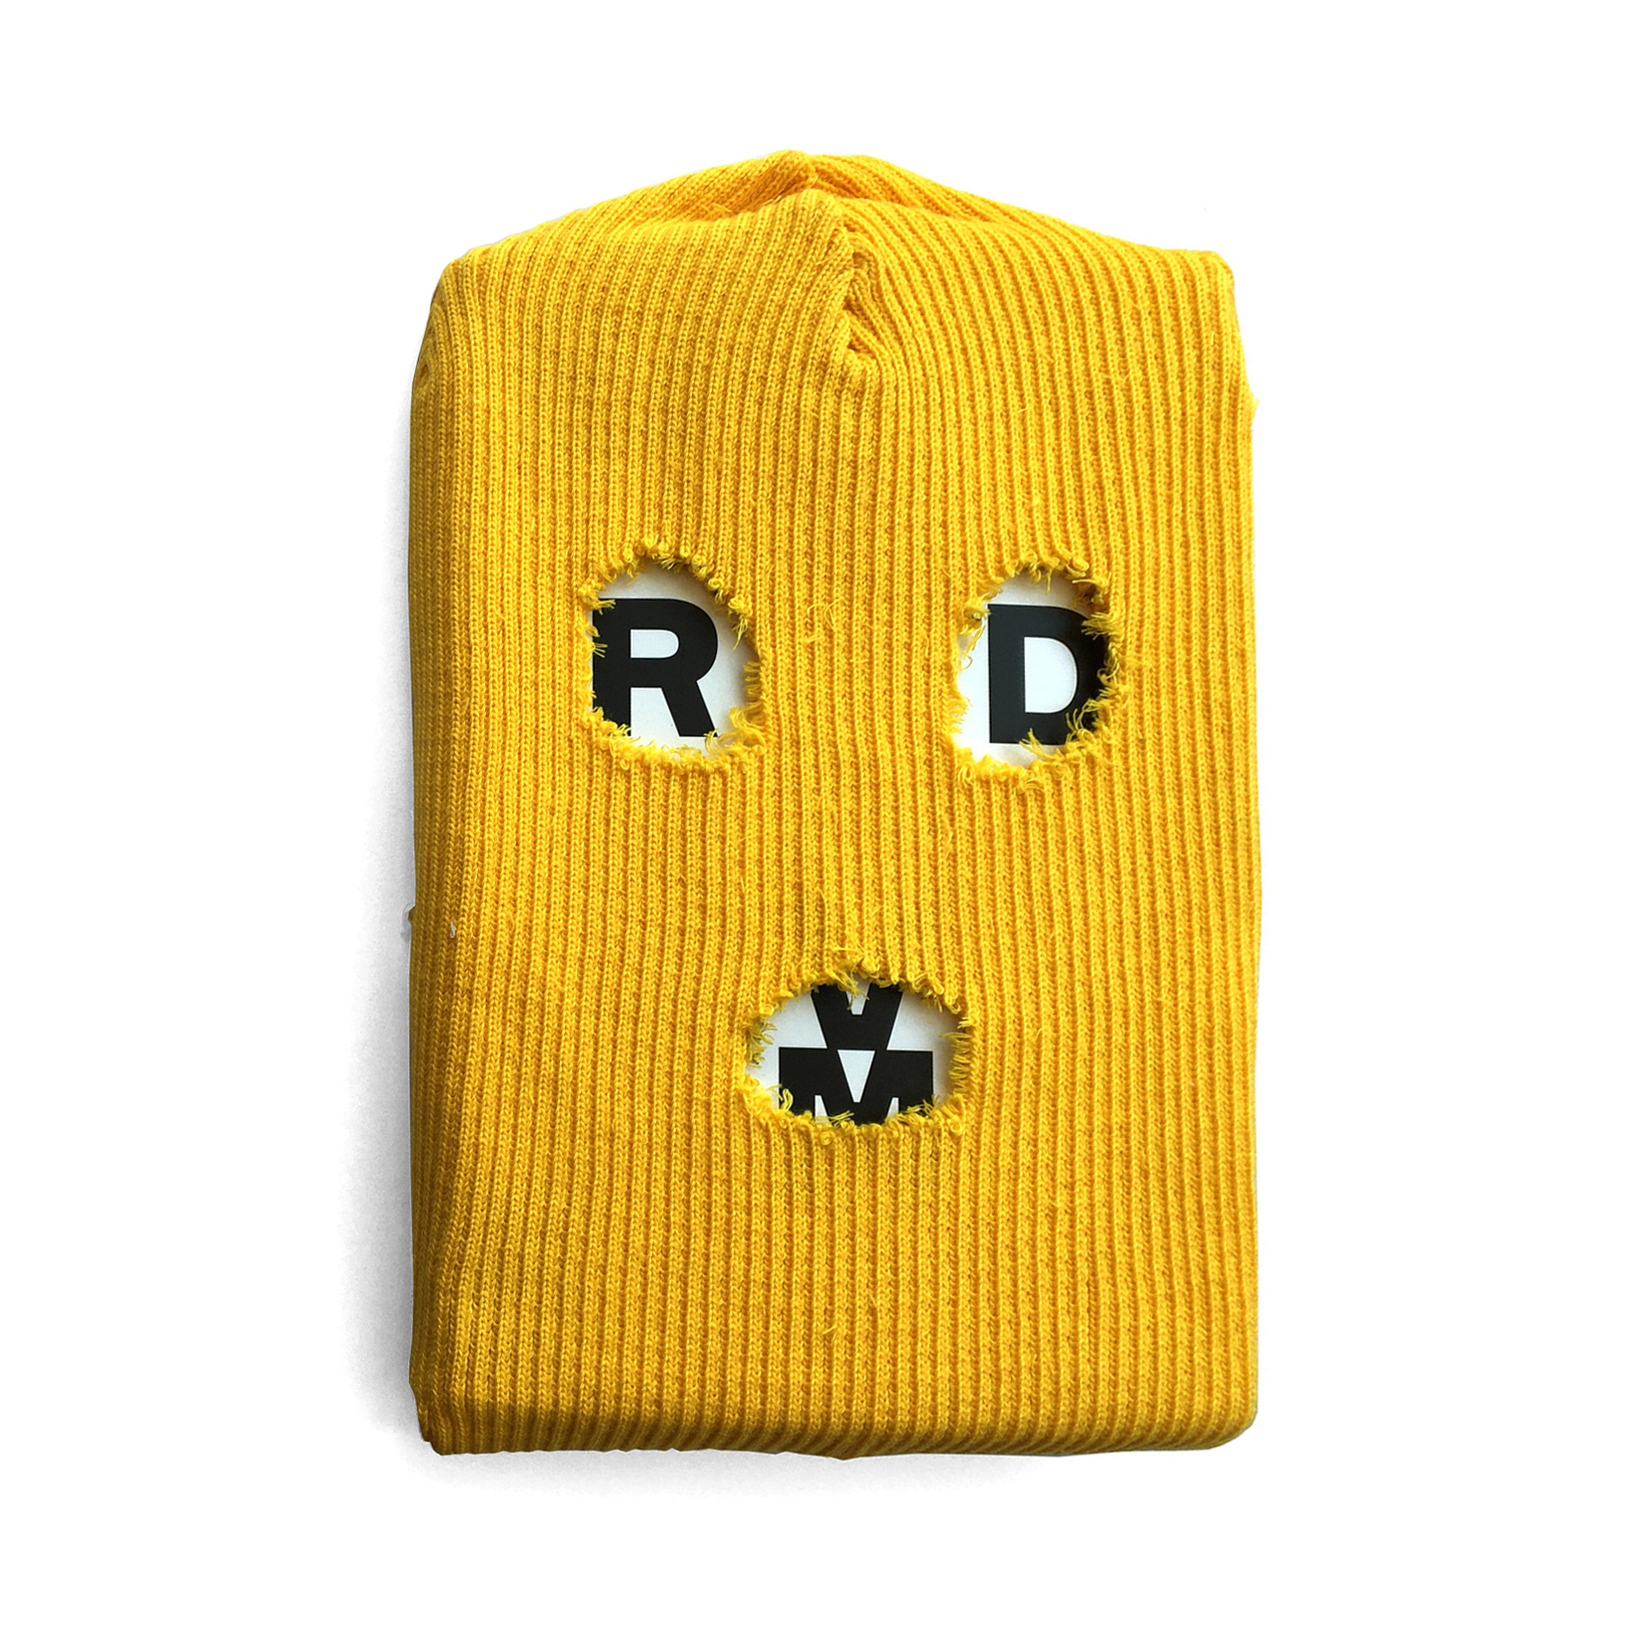
\includegraphics[width=46mm]{./grid/riot.jpg}}
\subfloat{
\includegraphics[width=46mm]{./grid/butler.png}}
\subfloat{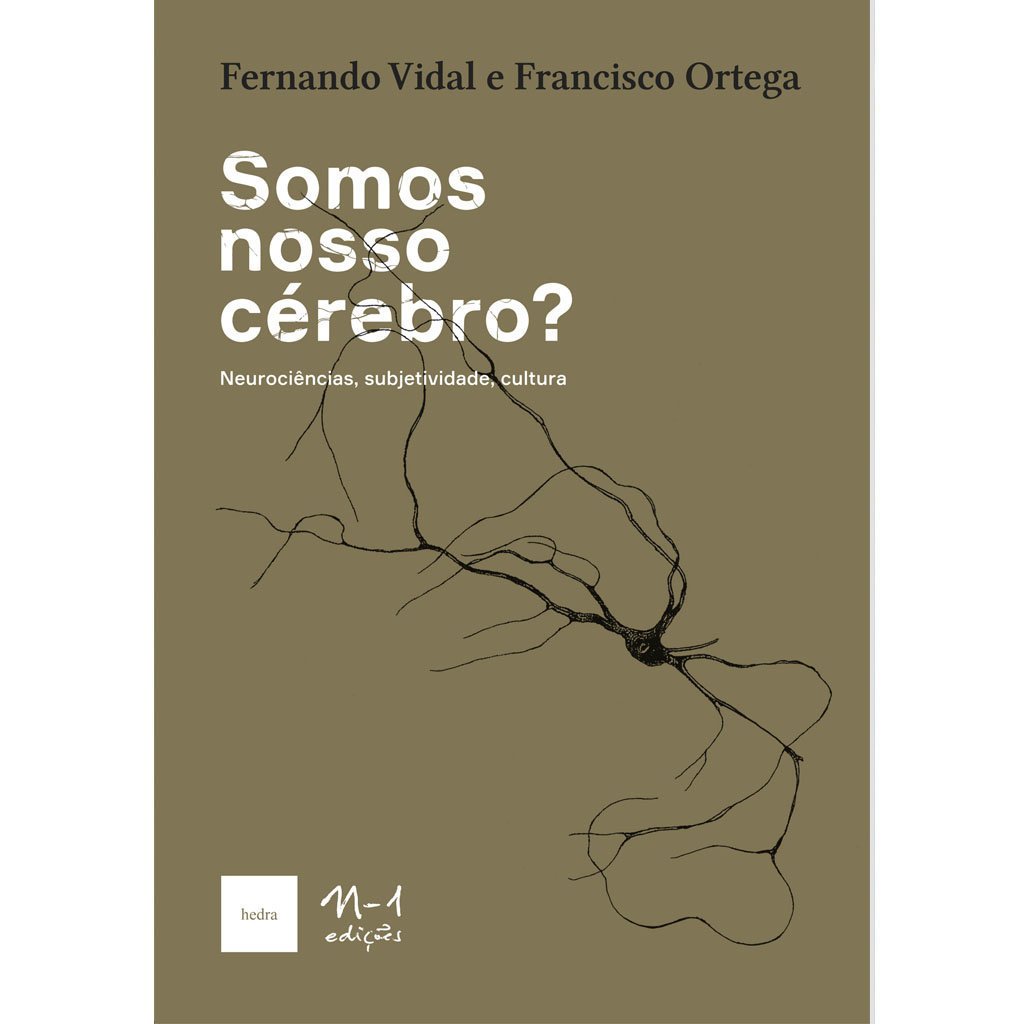
\includegraphics[width=46mm]{./grid/cerebro.png}}\\\hspace*{-.5cm}
\vspace{.5cm}
\subfloat{
\includegraphics[width=46mm]{./grid/gozo.jpg}}
\subfloat{
\includegraphics[width=46mm]{./grid/lazzarato.png}}
\subfloat{
\includegraphics[width=46mm]{./grid/coruja.jpg}}\\
\end{tabular}
\end{figure}

\pagebreak

\begin{figure}[!htbp]
\begin{tabular}{cccc}

\vspace{.5cm}
\hspace*{-.5cm}
\subfloat{
\includegraphics[width=46mm]{./grid/barricada.png}}
\subfloat{
\includegraphics[width=46mm]{./grid/cover.jpg}}
\subfloat{
\includegraphics[width=46mm]{./grid/lugares.jpg}}\\\hspace*{-.5cm}
\vspace{.5cm}
\subfloat{
\includegraphics[width=46mm]{./grid/1967.png}}
\subfloat{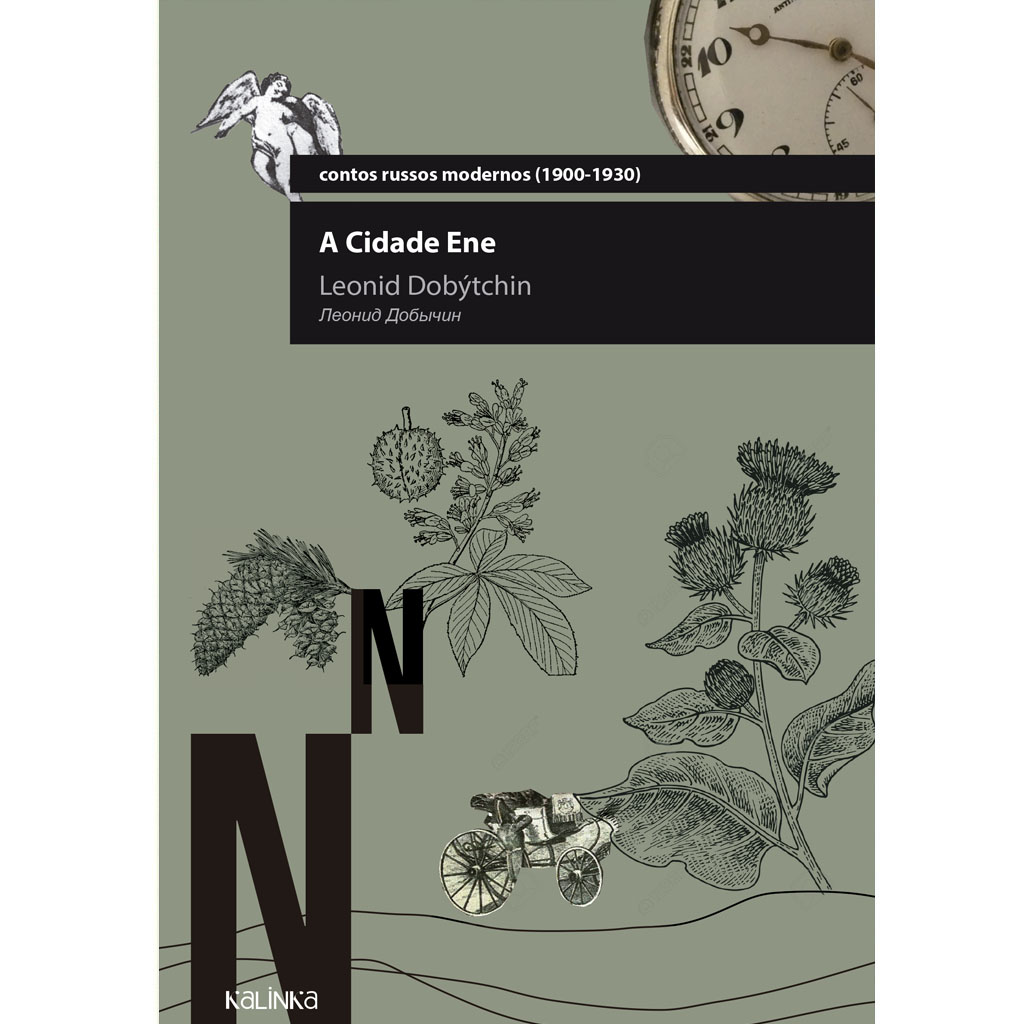
\includegraphics[width=46mm]{./grid/cidaden.jpg}}
\subfloat{
\includegraphics[width=46mm]{./grid/vagabond.jpg}}\\\hspace*{-.5cm}
\vspace{.5cm}
\subfloat{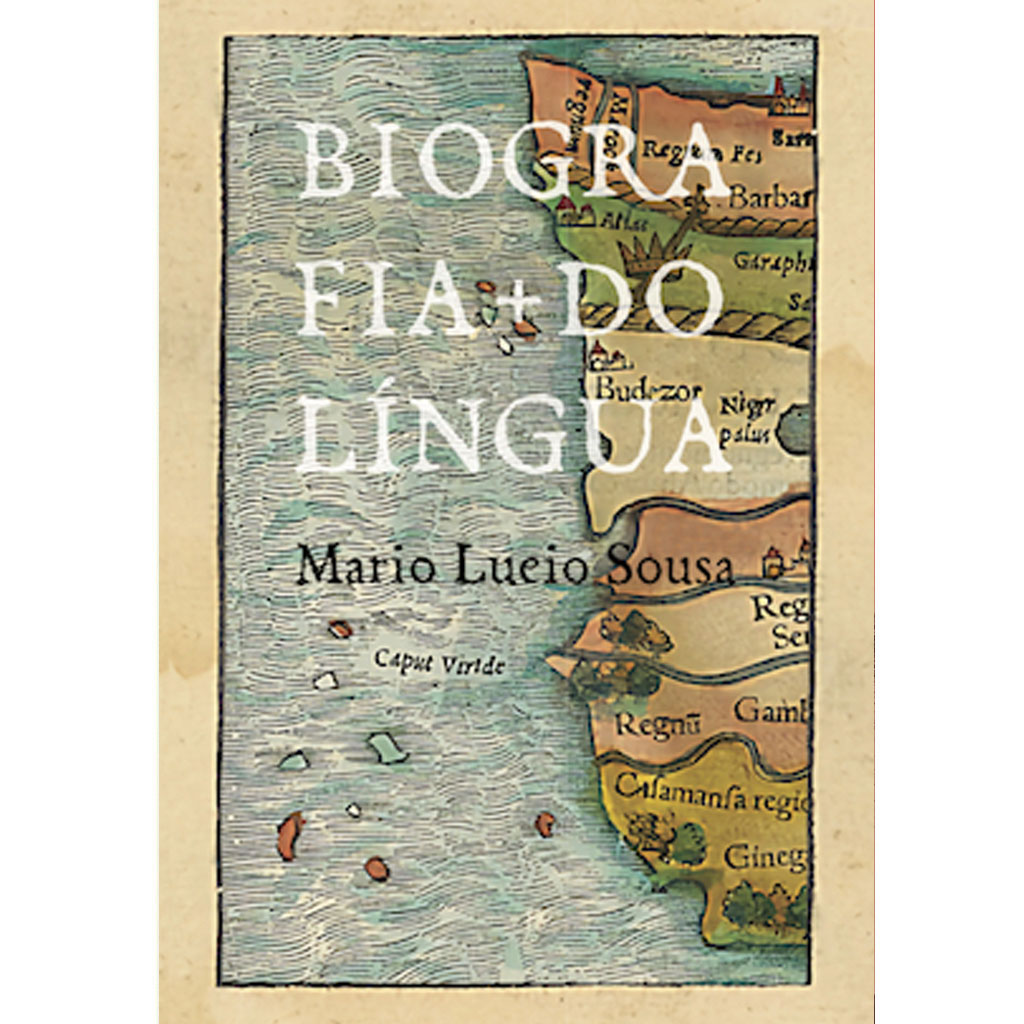
\includegraphics[width=46mm]{./grid/lingua.jpg}}
\subfloat{
\includegraphics[width=46mm]{./grid/luta.jpg}}
\subfloat{
\includegraphics[width=46mm]{./grid/cabalat.png}}\\\hspace*{-.5cm}
\vspace{.5cm}
\subfloat{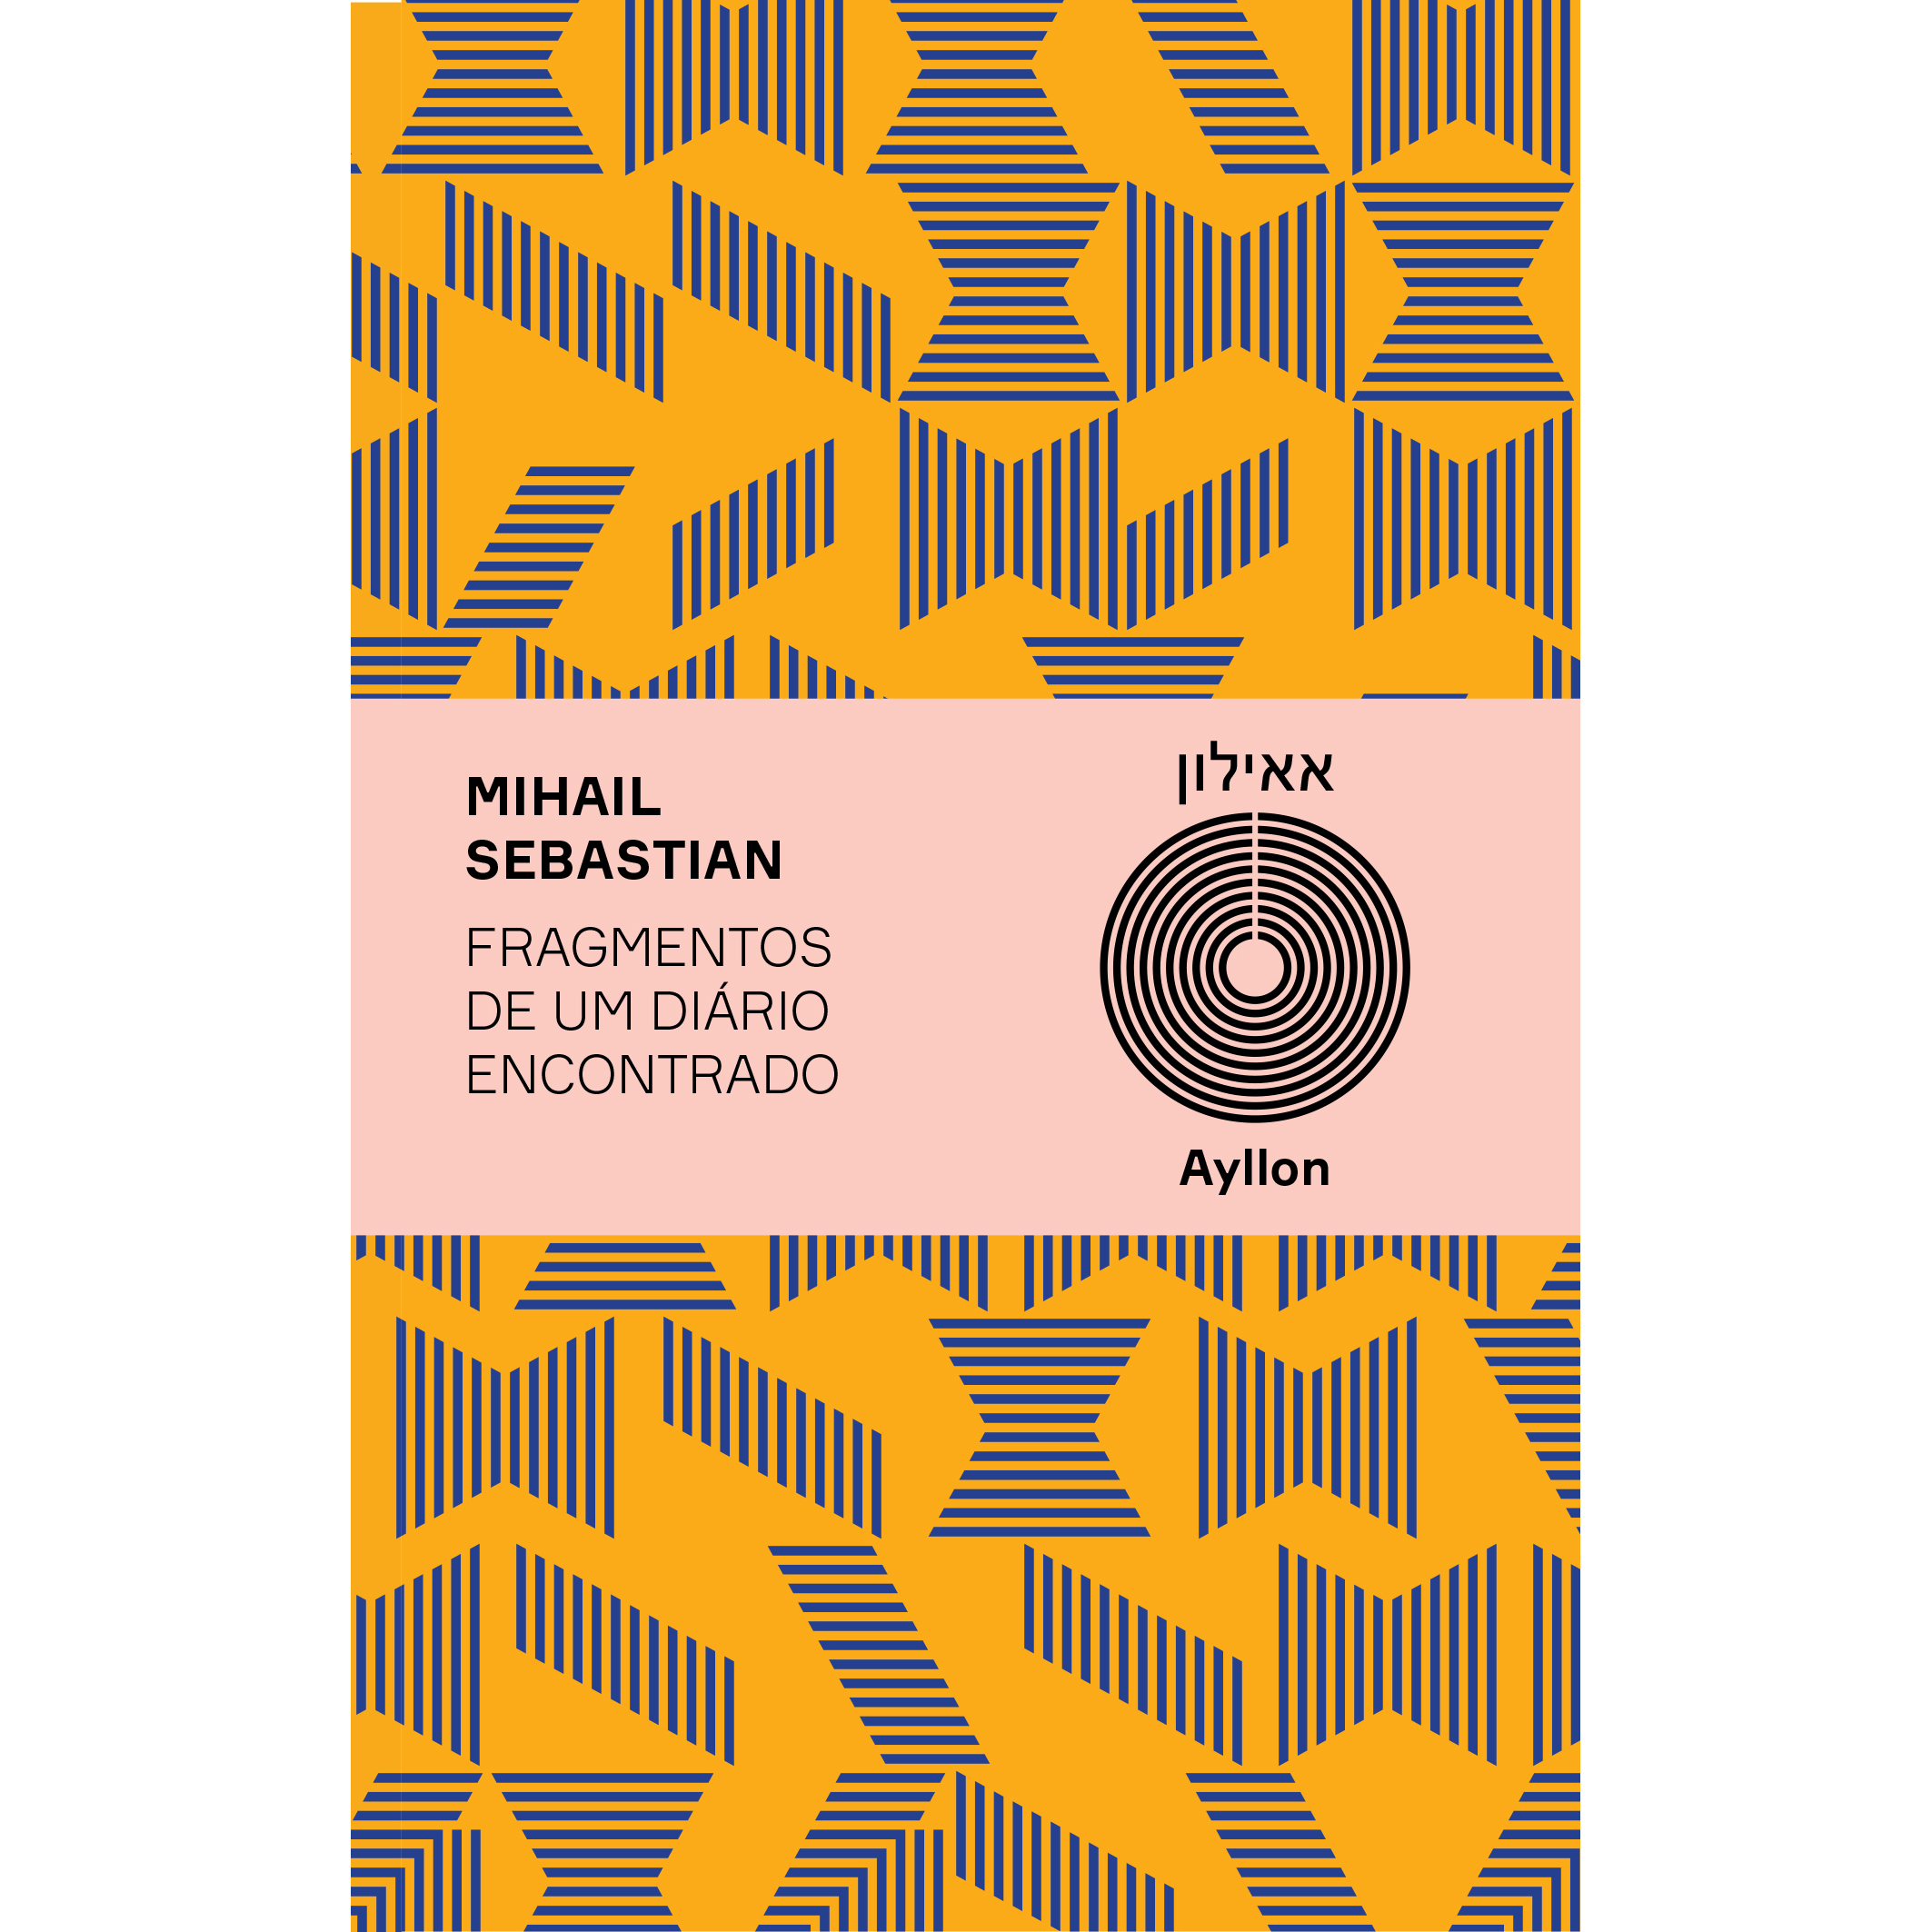
\includegraphics[width=46mm]{./grid/sebastian.jpg}}
\subfloat{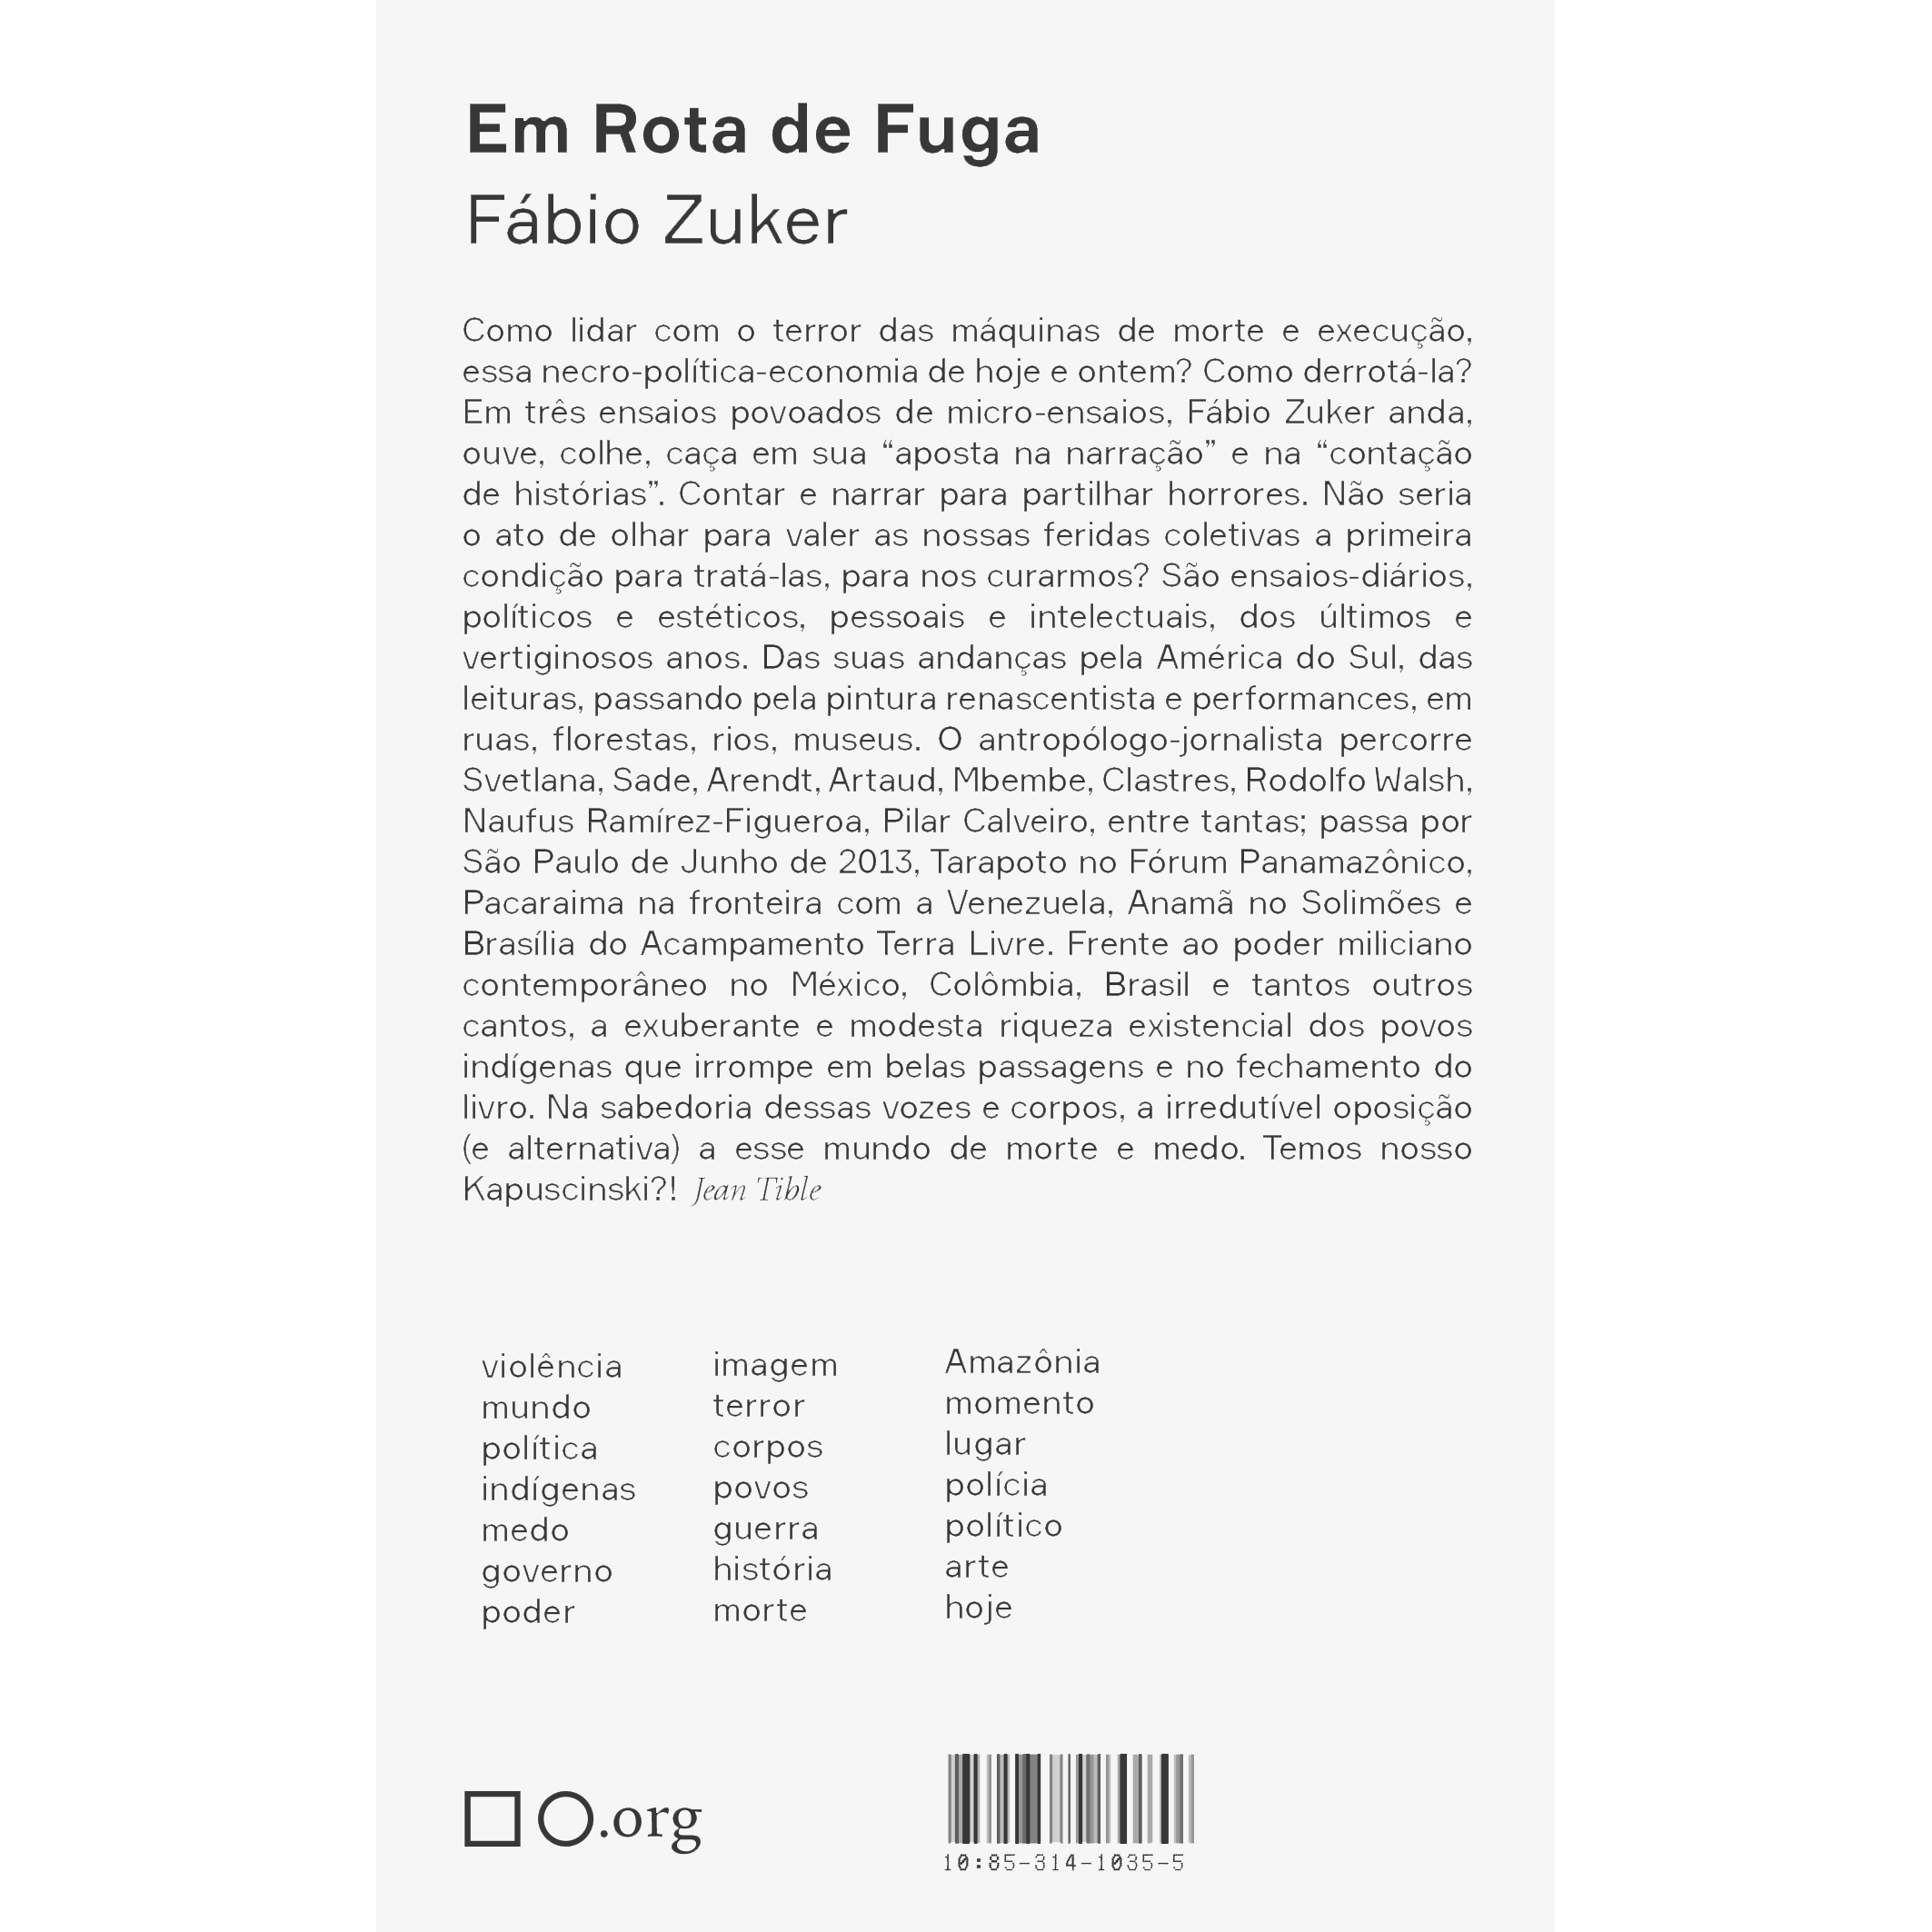
\includegraphics[width=46mm]{./grid/zuker.jpg}}
\subfloat{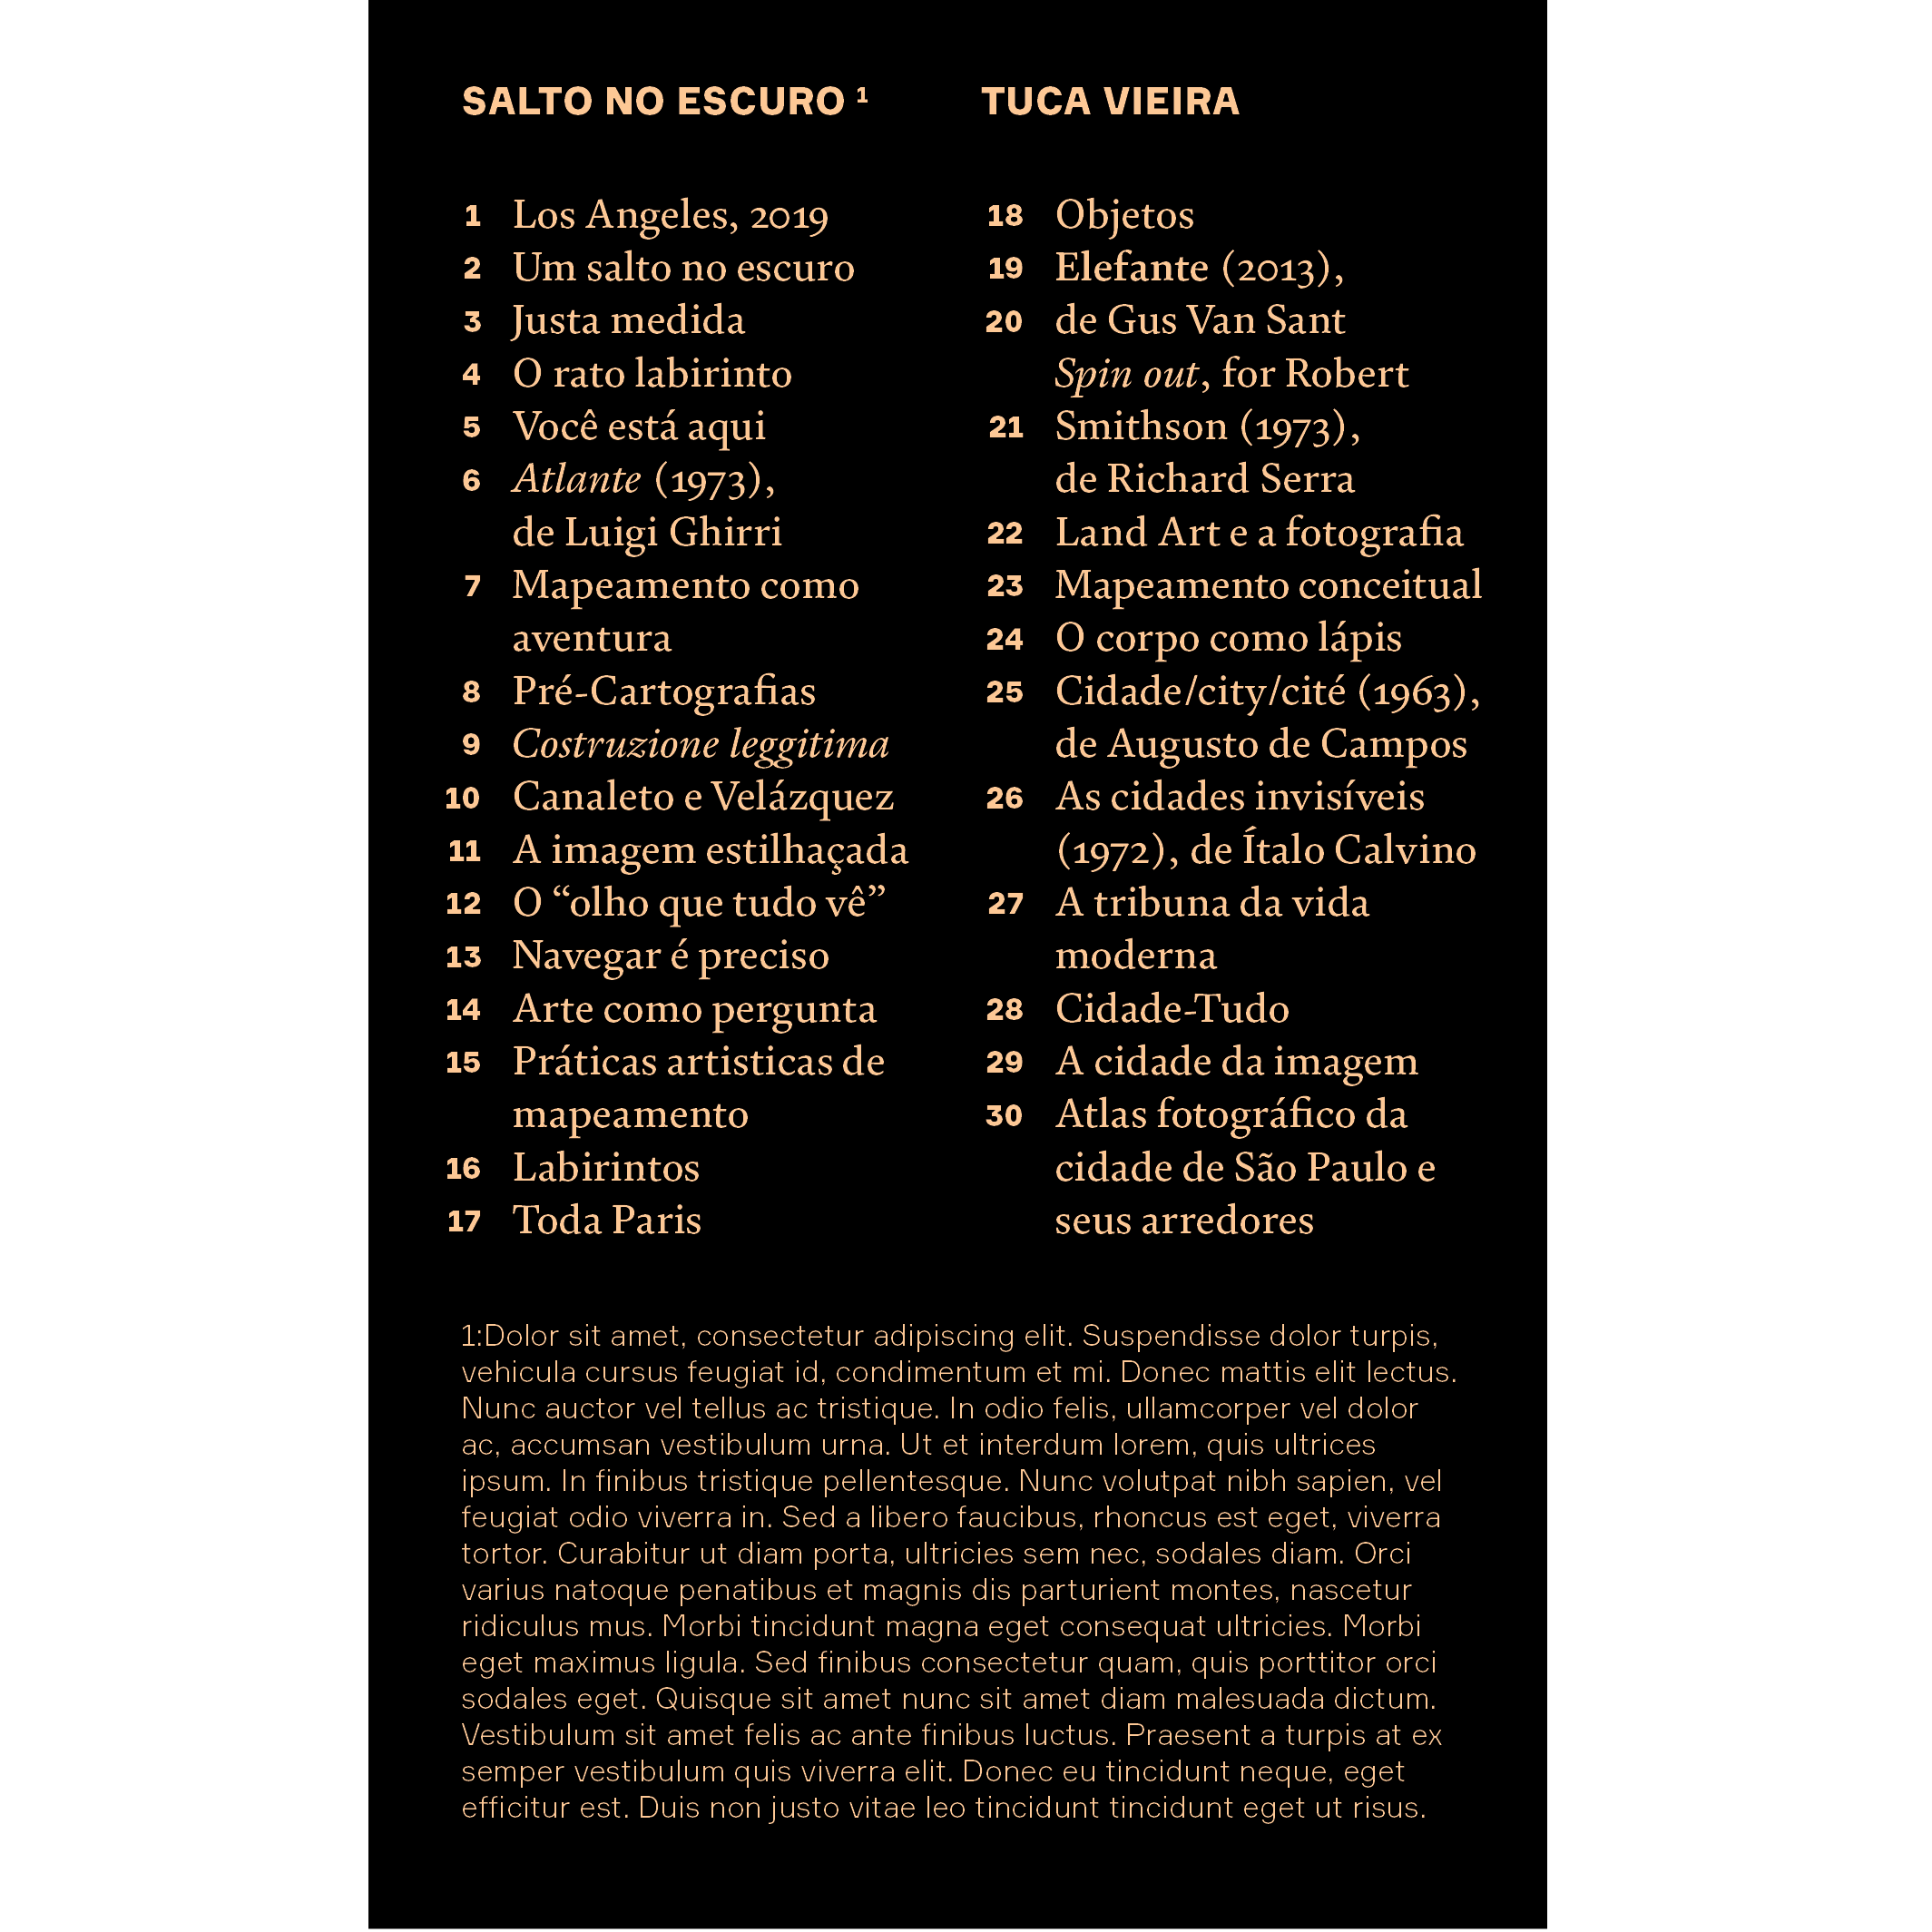
\includegraphics[width=46mm]{./grid/tuca.png}}\\
\end{tabular}
\end{figure}

\pagebreak

%\vspace*{.1cm}
%
%\begin{figure}[!htbp]
%\begin{tabular}{cccc}
%
%\vspace{.5cm}
%\hspace*{-.5cm}
%\subfloat{
\includegraphics[width=46mm]{./grid/tembeta.jpg}}\\\hspace*{-.5cm}
%\subfloat{\includegraphics[width=46mm]{./grid/mautner.jpg}}
%\subfloat{\includegraphics[width=46mm]{./grid/lage.jpg}}
%\subfloat{\includegraphics[width=46mm]{./grid/hotel.jpg}}
%
%\end{tabular}
%\end{figure}
%
%\pagebreak